\documentclass[12pt,a4paper]{report}

\usepackage{graphicx}
\usepackage{ragged2e}
\usepackage{geometry}
\usepackage{setspace}
\usepackage{comment}
\usepackage{biblatex}
\usepackage{hyperref}
\usepackage{fancyvrb}
\usepackage{caption}
\usepackage{amsmath}
\usepackage{float}
\usepackage{listings}
\usepackage{adjustbox}
\addbibresource{sample.bib}

\geometry{
 a4paper,
 total={170mm,257mm},
 left=25mm,
 right=25mm,
 top=20mm,
 }

\newcommand\myrepeat[2]{%
  \begingroup
  \lccode`m=`#2\relax
  \lowercase\expandafter{\romannumeral#1000}%
  \endgroup
}
\linespread{1.213}
\begin{document}
\begin{comment}Copertă 
\end{comment}
\begin{titlepage}
	\centering
	{\scshape\large \textbf{UNIVERSITATEA "ALEXANDRU IOAN CUZA" DIN IAȘI} \par}
	\vspace{0.5cm}
	{\scshape\Large \textbf{FACULTATEA DE INFORMATICĂ}\par}
	\vspace{2cm}
	
\includegraphics[width=0.15\textwidth]{logo-fii}\par\vspace{1cm}
	{\scshape\normalsize LUCRARE DE LICENȚĂ\par}
	\vspace{1cm}
	{\huge\bfseries Gemixque\par}
	\vspace{1cm}
	{\normalsize \textbf{sistem de recomandări de jocuri video}\par}
	\vspace{1.5cm}
	{\normalsize \textbf{propusă de}\par}
	\vspace{1cm}
	{\Large\itshape\textbf {Radu Damian}\par}
	\vspace{2cm}
	{\normalsize \textbf{Sesiunea:} \textit{iunie/iulie, 2022}\par}
	\vspace{1cm}
	{\normalsize \textbf{Coordonator științific}\par}
	\vspace{0.5cm}
	{\Large\itshape\textbf {Lect.dr. Cristian Frăsinaru}\par}
\end{titlepage}

\begin{comment}Prima pagină
\end{comment} 
\begin{titlepage}
	\centering
	{\scshape\large \textbf{UNIVERSITATEA "ALEXANDRU IOAN CUZA" DIN IAȘI} \par}
	\vspace{0.5cm}
	{\scshape\Large \textbf{FACULTATEA DE INFORMATICĂ}\par}
	\vspace{5cm}


	{\huge\bfseries Gemixque\par}
	\vspace{1cm}
	{\normalsize \textbf{sistem de recomandări de jocuri video}\par}
	\vspace{3cm}
	{\Large\itshape\textbf {Radu Damian}\par}
	\vspace{2cm}
	{\normalsize \textbf{Sesiunea:} \textit{iunie/iulie, 2022}\par}
	\vspace{4cm}
	{\normalsize \textbf{Coordonator științific}\par}
	\vspace{0.5cm}
	{\Large\itshape\textbf {Lect.dr. Cristian Frăsinaru}\par}
\end{titlepage}

\begin{comment}Declarație standard privind originalitatea lucrării
\end{comment}
\begin{titlepage} 


	\begin{FlushRight}Avizat,\end{FlushRight}
	\begin{FlushRight}Îndrumător Lucrare de Licență				\end{FlushRight}
	\begin{FlushRight}Titlul, Numele și Prenume \hspace{2em}	\rule{5cm}{0.15mm}
	\end{FlushRight}

	\begin{FlushRight}Data \rule{2cm}{0.15mm} \hspace{2em} 	Semnătura \rule{2cm}{0.15mm} \end{FlushRight}

	\hfill \break

	\begin{center}
	\textbf{DECLARAȚIE privind originalitatea conținutului 	lucrării de licență}
	\end{center}
	
	
	\justifying
	\hspace{1em} Subsemnatul(a) \hspace{1em} \myrepeat{90}{.} \newline
	domiciliul în \myrepeat{90}{.} \newline
	născut(ă) la data de \myrepeat{30}{.},\hspace{1em} identificat prin CNP 
\myrepeat{40}{.},
	absolvent(a) al(a) Universității "Alexandru Ioan Cuza" din Iași, \newline
	 Facultatea de \myrepeat{30}{.} \hspace{1em} specializarea \hspace{1em} \myrepeat{55}{.},
	 promoția \hspace{1em} \myrepeat{30}{.}, declar pe propria
	 răspundere, cunoscând consecințele \newline falsului în
	 declarații în sensul art. 326 din Noul Cod Penal și 
	 dispozițiile Legii Educației Naționale nr. 1/2011
	 art.143 al. 4 si 5 referitoare la plagiat, că lucrarea de
	 licență cu titlul: \rule{16cm}{0.15mm} \newline
	 \rule{16cm}{0.15mm} \newline
	 elaborată sub îndrumarea dl. / d-na \rule{9.3cm}{0.15mm}
	 \newline pe care urmează să o susțină în fața
	 comisiei este originală, îmi aparține și îmi asum 				 conținutul său în întregime. 
	 
	 \hspace{1em} De asemenea, declar că sunt de acord ca
	 lucrarea mea de licență să fie verificată prin orice
	 modalitate legală pentru confirmarea originalității,
	 consimțind inclusiv la introducerea conținutului său
	 într-o bază de date în acest scop.
	 
	 \hspace{1em} Am luat la cunoștință despre faptul că este interzisă
	 comercializarea de lucrări științifice în vederea
	 facilitării falsificării de către cumpărător a calității
	 de autor al unei lucrări de licență, de diplomă sau de
	 disertație în acest sens, declar pe proprie răspundere
	 că lucrarea de față nu a fost copiată ci reprezintă rodul 
	 cercetării i pe care am întreprins-o.
	 
	 \hfill \break
	 
	 \hspace{1em} Dată azi, \myrepeat{30}{.}
	 \hspace{5em} Semnătură student \myrepeat{30}{.}
	 
\end{titlepage}

\begin{comment}Declarație standard privind drepturile de utilizare a lucrării și a codului sursă
\end{comment}
\begin{titlepage}
	\hfill \break
	\begin{center}
	DECLARAȚIE DE CONSIMȚĂMÂNT
	\end{center}
	
	\hfill \break
	\justifying
	Prin prezenta declar că sunt de acord ca Lucrarea de
	licență cu titlul \emph{"Gemixque"},
	codul sursă al programelor și celelalte conținuturi
	(grafice, multimedia, date de test etc.) care însoțesc
	această lucrare să fie utilizate în cadrul Facultății
	de Informatică.
	
	De asemenea, sunt de acord ca Facultatea de Informatică
	de la Universitatea "Alexandru Ioan Cuza" din Iași,
	să utilizeze, modifice, reproducă și să distribuie în
	scopuri necomerciale programele-calculator, format
	executabil și sursă, realizate de mine în cadrul prezentei
	lucrări de licență.
	
	\hfill \break
	\hfill \break
	\hfill \break
	\hfill \break
	\hfill \break
	Iași, \emph{data}
	
	\hfill \break
	\hfill \break
	\hfill \break
	\hfill \break
	\hfill \break
	\begin{FlushRight}Absolvent  \emph{Radu Damian} \end{FlushRight}
	\begin{FlushRight}\rule{4.5cm}{0.15mm} \end{FlushRight}
	\begin{FlushRight}(semnătura în original) \end{FlushRight}
	
	
\end{titlepage}

\hfill \break
	\begin{center}
	{\scshape\large \textbf{Mulțumiri} \par}
	\end{center}
	
\begin{flushright}
\hfill \break
\hfill \break
Sunt profund recunoscător pentru sprijinul necondiționat oferit de părinții și de bunica mea în vederea realizării acestei lucrări de licență.
\end{flushright}
\hfill \break
\hfill \break
\hfill \break
\begin{flushright}
Îi mulțumesc Monicăi pentru faptul că m-a ajutat să-mi gestionez trăirile și să privesc provocările pe care le-am întâmpinat cu o atitudine sănătoasă.
\hfill \break
\hfill \break
\hfill \break
\end{flushright}
\begin{flushright}
De asemenea, îi mulțumesc domnului prof. dr Frăsinaru Cristian, îndrumător al lucrării de licență, pentru sfaturile, resursele, și încrederea oferită de-a lungul perioadei în care am lucrat pentru licență.
\end{flushright}

\newpage
   
\renewcommand*{\contentsname}{Cuprins}
\tableofcontents
\newpage

\hfill \break

	\hfill \break
	\begin{center}
	{\scshape\large \textbf{Introducere} \par}
	\end{center}
	
	Această lucrare de licență propune prezentarea implementării unui sistem de recomandare, sub forma unei aplicații web.
	
	În următoarele capitole vor fi ilustrate următoarele: problema ce trebuie rezolvată, tehnologiile folosite, modelarea bazei de date, modul în care au fost generate datele de intrare ale problemei, server-ul de back-end, algoritmul implementat și server-ul de front-end.
	
	\begin{center}
	{\scshape\large \textbf{Motivație} \par}
	\end{center}

	Ideea de bază a lucrării de licență a venit oarecum din întâmplare. Când eram student în semestrul II din anul 2 de facultate, mă uitasem într-o zi obișnuită la acest site: \href{https://simkl.com/}{https://simkl.com}, pe care-l foloseam pentru a nu uita la ce episod am rămas dintr-un anumit serial. Acest site poate oferi și recomandări de filme/seriale în funcție de datele din profilul meu.
	
	Fiind un amator de jocuri video pe PC, mi-a venit ideea de a face un astfel de site, însă care să recomande, bineînțeles, jocuri video.
	
	O observație importantă este faptul că aș fi putut alege orice resursă ce poate fi recomandată(de exemplu: periuțe de dinți, telefoane, picturi etc.), așadar problema în speță poate fi privită într-un mod mai general. Motivul pentru care am ales jocurile video este dat de pasiunea mea pentru acestea.
	
	De asemenea, eram curios în acea perioadă, printre altele, legat de cum aș putea implementa o soluție pentru acest sistem de recomandare pe care mi l-am propus să-l realizez.
	
	Așadar, am avut inspirație, dar și noroc, deoarece această idee mi-a venit relativ repede, lucru ce a reprezentat un punct de pornire important în realizarea efectivă a acestei lucrări.
	
	\newpage
	
	\begin{center}
	{\scshape\large \textbf{Aplicații similare} \par}
	\end{center}
	
	Din aplicațiile similare căutate, am identificat următoarele pe care le-am considerat mai notabile:
	
\begin{itemize}
  \item IGDB - \url{https://www.igdb.com/}
  \item Steam - \url{https://store.steampowered.com/}
  \item Metacritic - \url{https://www.metacritic.com/}
  \item Quantic Foundry - \url{https://quanticfoundry.com/}
  \item Games finder - \url{https://gameslikefinder.com/}
\end{itemize}


Încercând să caut informații legate de modul concret de implementare al recomandărilor care se regăsesc în aceste aplicații, mi-am dat seama că acest lucru este în zadar, din cauza aspectului comercial al aplicațiilor.

Chiar și așa, aplicația ce va fi prezentată în această lucrare de licență are un algoritm de recomandare ce a necesitat o documentare în prealabil, și utilizează de asemenea o bază de date nerelațională de tip graf.

Așadar, aplicația propusă s-ar putea descrie mai degrabă ca o tentativă de a îmi răspunde la următoarea întrebare care nu mi-a fost răspunsă consultând aplicațiile similare: Cum se poate implementa un algoritm de recomandare?

Bineînțeles că răspunsul nu este unul universal, ci propun o variantă(din nenumăratele care pot exista, căci este loc de inovații și contribuții semnificative în a ataca această problemă) care a fost șlefuită folosind resurse proprii.

În timpul implementării aplicației, mi-am dat seama că răspunsul meu poate fi privit doar ca un punct de pornire pentru a dezvolta în continuare partea de recomandare a aplicației. Aceste reflecții pot fi regăsite în capitolul \textbf{Concluzii și direcții viitoare}.
	
	
\newpage
	
\setcounter{secnumdepth}{3} 
\renewcommand*\thesection{\arabic{section}}
\section{Descrierea problemei}

Problema ce trebuie rezolvată se rezumă la recomandarea unor jocuri video(niciunul, unul, sau mai multe) unui utilizator. În ansamblu, datele de intrare ar putea fi reprezentate de o mulțime de jocuri video, o mulțime de utilizatori și o mulțime de recenzii.

Aceste recenzii sunt oferite de utilizator și asociate unui joc. În recenzie, utilizatorul oferă o notă(un scor, pe o scară de la 1 la 10) care indică cât de mult i-a plăcut/displăcut jocul respectiv. Un utilizator poate face maxim o recenzie per joc.

O descriere mai amănunțită a utilizatorilor, recenzilor și a jocurilor se poate regăsi în capitolul 4 \textbf{Baza de date}, subcapitolul \textbf{Modelarea bazei de date}.

\subsection{Scopuri și cerințe ale aplicației}

\bigskip
\bigskip
\textbf{Scopul documentului}
\bigskip

Scopul acestui document este de a ilustra modul în care funcționează un sistem de recomandări de jocuri video sub forma unei aplicații web având ca soluție de stocare o bază de date de tip graf NoSql.

\bigskip
\textbf{Publicul țintă}
\bigskip

Acest document este destinat atât cititorilor avizați(e.g. profesori universitari) pentru a afla de exemplu soluțiile utilizate în cadrul capitolelor 4, 5 sau 6, \textbf{Baza de date}, \textbf{Back-end} respectiv \textbf{Algoritmul de recomandare}, cât și cititorilor neavizați(utilizatori obișnuiți), care se pot informa în legătură cu modul în care pot interacționa cu site-ul în capitolul 8 \textbf{Manual de utilizare}.

\bigskip
\textbf{Scopul aplicației}
\bigskip

Scopul acestei aplicații este de a oferi o soluție în a contracara cantitatea masivă de informații ce se regăsește pe internet \cite{5} în ceea ce privește multitudinea de jocuri video, prin a dezvolta un sistem de recomandări care să faciliteze decizia unui utilizator legat de ce joc să aleagă.

\bigskip
\textbf{Contribuții}
\bigskip  

Generarea datelor de intrare ale problemei a fost realizată de mine, în sensul că nu am folosit în mod direct seturi de date externe(de exemplu: Kaggle), ci am implementat un modul în Java care generează fișiere tip csv.

De asemenea, implementarea algoritmului a fost făcută fără utilizarea unei librării externe(cum s-ar fi putut face de exemplu cu Python). Motivația acestei decizii este reprezentată de a avea o perspectivă mai profundă a unui posibil algoritm de recomandare.

\section{Tehnologii folosite}

Pentru aplicația web:

\begin{enumerate}
  \item Baza de date: Neo4j.
  \item Server de back-end:
  \begin{itemize}
     \item Limbaj: Java versiunea 11
     \item Framework: Spring Boot
     \item REST API
   \end{itemize}
  \item Server de front-end:
  \begin{itemize}
     \item Limbaj: Typescript
     \item Framework: Angular
   \end{itemize}
\end{enumerate}
Pentru modulul de generare al datelor de intrare:

\begin{enumerate}
  \item API extern folosit pentru a procura date despre jocuri video: IGDB API \cite{1}
  \item API extern folosit pentru procurarea de recenzii de pe Steam \cite{2}
  \item Java Faker - pentru generarea de date aleatoare \cite{3}
  \item Apache Commons CSV - pentru manipularea de fișiere CSV \cite{4}
\end{enumerate}

\newpage

\section{Arhitectura sistemului}

Arhitectura sistemului ce propune rezolvarea problemei este următoarea:

\begin{figure}[H]
\centering
\caption{}
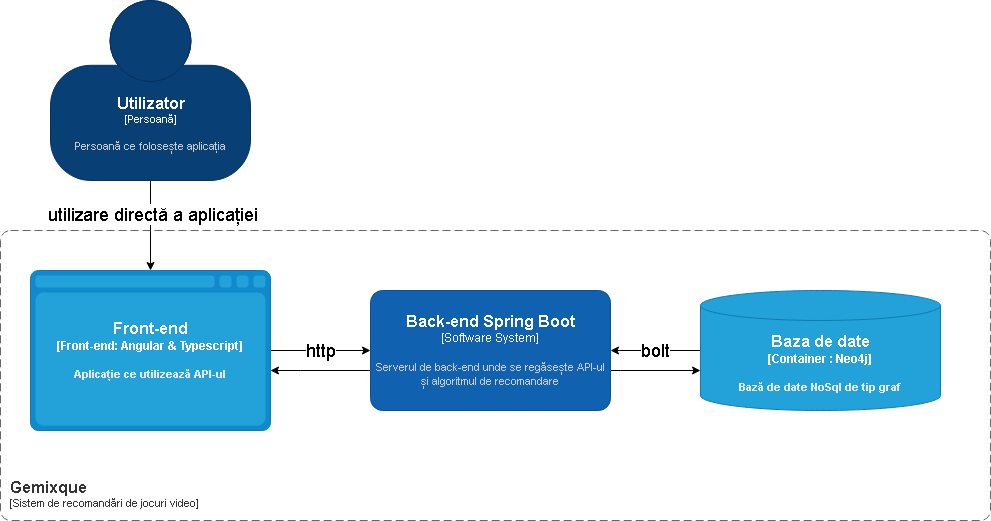
\includegraphics[scale = 0.5]{exemplu_17_diagrama_c4_nivel_1.drawio}
\caption*{Diagramă C4 nivelul 1}
\end{figure}

Se poate observa în ansamblu suita de tehnologii folosite: Neo4j pentru baza de date, Spring Boot pentru back-end și Angular pentru front-end.

Schema bazei de date va fi reprezentată în capitolul următor, deoarece înțelegerea acesteia presupune o scurtă inițiere în ceea ce propune Neo4j.

\newpage


\section{Baza de date}
\subsection{Introducere}

Tipul de stocare ales este cel oferit de Neo4j, în care se prezintă o abordare NoSQL de tip graf.  Comparativ cu o bază de date relațională, în care datele sunt stocate prin intermediul unor înregistrări(tuple) în tabele, în Neo4j datele sunt stocate prin intermediul nodurilor și muchiilor.

În exemplul următor, vor fi ilustrate caracteristicile nodurilor și muchiilor în stocarea efectivă a datelor:


\begin{figure}[H]
\centering
\caption{}
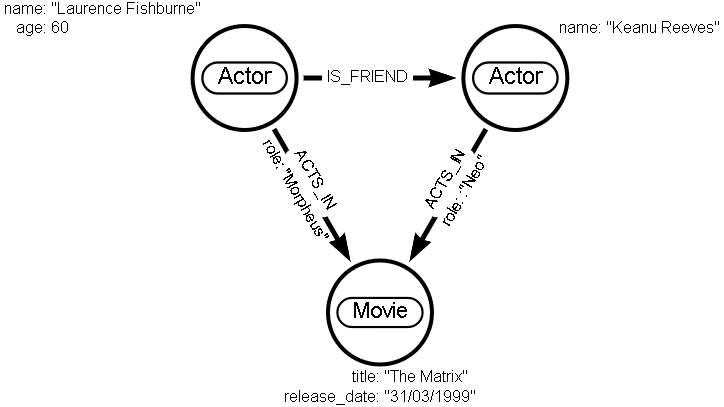
\includegraphics[scale=0.5]{exemplu_1_neo4j}
\caption*{}
\end{figure}


Un nod în neo4j are următoarele caracteristici \cite{6}: reprezintă entități/obiecte, pot fi etichetate și pot avea proprietăți.

Observăm din figură cele trei entități: două noduri etichate cu 'Actor' și un nod etichetat cu 'Movie'. De asemenea, ambele noduri 'Actor' au proprietatea 'name', însă doar unul din ele are și proprietatea 'age'. Așadar, nu trebuie neapărat ca două noduri cu aceeași etichetă să aibă aceleași proprietăți.

Încă un lucru important de menționat este faptul că un nod poate avea mai multe etichete, așa cum se poate vedea din următorul exemplu:


\begin{figure}[H]
\centering
\caption{}
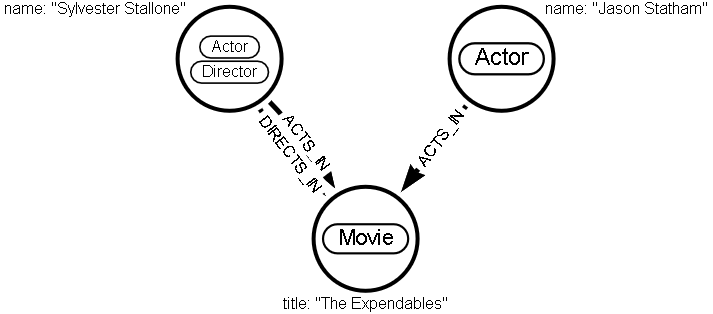
\includegraphics[scale=0.5]{exemplu_2_neo4j}
\caption*{}
\end{figure}


Practic, din această figură se observă faptul că se poate modela cu ușurință situația în care un regizor joacă în propriul său film.

O altă noțiune importantă într-o bază de date de tip graf este cea de relație, care este asociată unei muchii. 
O relație trebuie să aibă un tip, un sens, și poate avea proprietăți.
Din figurile anterioare s-au putut observa relațiile \texttt{ACTS\_IN}, \texttt{DIRECTS\_IN} sau \texttt{IS\_FRIEND}.

Un alt aspect important de precizat este faptul că între două entități pot exista mai multe relații, așa cum s-a putut vedea în figura anterioară. Așadar, se modelează practic un multigraf orientat.

\subsection{De ce NoSQL și nu SQL?}

Având în vedere faptul că în această aplicație este prezentă o rețea socială în care mai mulți utilizatori pot interacționa între ei și pot oferi recenzii jocurilor video, o bază de date de tip graf este o alegere inspirată.

În ceea ce privește limbajul utilizat pentru a efectua interogări pe baza de date, avem în vedere următorul studiu de caz:

Să presupunem că dorim să modelăm ceea ce se întâmplă în cadrul unei facultăți, pe scurt: gestionarea studenților, a notelor pe care le iau aceștia la cursuri, și a profesorilor.
Exemplul ce urmează a fi ilustrat se bazează pe schema bazei de date ce a fost utilizată în cadrul materiei Baze de date din anul II semestrul I. \cite{7}

Să propunem că dorim să efectuăm următoarea interogare: pentru un student, să aflăm numele profesorilor la cursurile în care studentul a luat nota 10.

O interogare în limbajul SQL ar putea arăta în felul următor:

\begin{figure}[H]
\centering
\begin{BVerbatim}
SELECT p.nume, p.prenume FROM NOTE n 
JOIN CURSURI c ON n.id_curs = c.id
JOIN DIDACTIC d ON d.id_curs = c.id
JOIN PROFESORI p ON p.id = d.id_profesor
WHERE VALOARE = 10 AND ID_STUDENT = 36;
\end{BVerbatim}
\end{figure}


Se poate observa așadar faptul că sunt necesare o serie de join-uri pentru a putea obține rezultatul dorit.


Pentru a putea compara această interogare cu cea care s-ar putea face în limbajul Cypher folosit în Neo4j, se va ilustra pe scurt cum s-ar putea modela schema bazei de date anterior menționată în una de tip graf. (nu în totalitate, ci doar de ceea ce avem nevoie pentru a evidenția interogarea)


\begin{figure}[H]
\centering
\caption{Miniatură a schemei bazei de date}
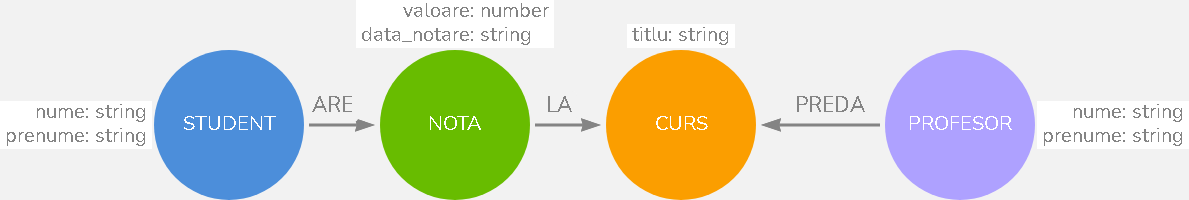
\includegraphics[scale=0.4]{exemplu_3_neo4j}
\caption*{}
\end{figure}


Așadar, având în vedere acest model, interogarea în Cypher ar putea arăta în felul următor:

\begin{figure}[H]
\centering
\begin{BVerbatim}
MATCH (s:STUDENT)-[:ARE]->(n:NOTA {valoare: 10}),
(n)-[:LA]->(:CURS)<-[:PREDA]-(p:PROFESOR)
WHERE id(s) = 0
RETURN p.nume, p.prenume
\end{BVerbatim}
\end{figure}



Un prim lucru interesant care s-ar putea observa este faptul că Cypher introduce prin sintaxa sa conceptul de ASCII Art \cite{8}, \cite{9}, care practic face posibilă o nouă interpretare a codului, una vizuală, adică se poate observa relativ ușor cum ceea ce este scris în primele două linii de cod seamănă destul de mult cu modelul din figura anterioară.
Cele două linii s-ar fi putut scrie într-o singură linie fără nicio dificultate, însă am optat pentru această variantă pentru o mai bună lizibilitate a codului.

Pe de altă parte, o altă caracteristică importantă a bazelor de date de tip graf este că relațiile între entități au cea mai mare prioritate în modelarea datelor \cite{10}, acest lucru reflectându-se în modul cum a fost construită această interogare, în care este mult mai facil să interogăm niște date aflate la capătul unui lanț format din mai multe relații, așa cum se observă și în acest exemplu.

Pentru o mai bună înțelegere a modului în care sunt reprezentate efectiv datele, se poate vedea figura de mai jos:

\begin{figure}[H]
\centering
\caption{}
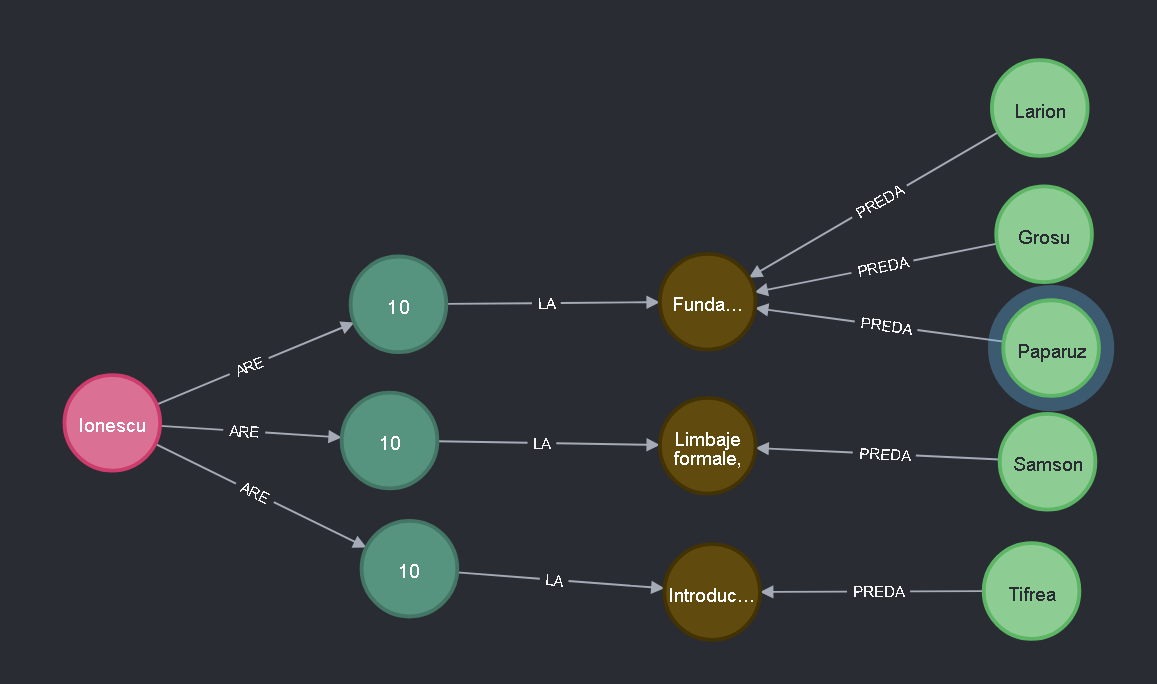
\includegraphics[scale=0.5]{exemplu_4_neo4j}
\caption*{Datele folosite pentru a exemplifica interogarea în Cypher}
\end{figure}

\subsection{Modelarea bazei de date}


Având în vedere noțiunile prezentate în capitolele anterioare, în acest capitol va fi descrisă schema bazei de date ce va fi folosită pentru a stoca datele necesare rezolvării problemei de a recomanda jocuri video.

Însă, înainte de a ilustra schema în ansamblu, fiecare entitate în parte va fi detaliată în rândurile următoare.

\bigskip
\textbf{Utilizatorul}
\bigskip

Această entitate reprezintă punctul central al aplicației, deoarece utilizatorul este cel care oferă recenzii(note) jocurilor și influențează într-un mod indirect recomandările unui alt utilizator, deci el este cel care, practic, inițiază acțiunea.

Nodul corespunzător acestei entități este cel din \textbf{Figura 5}.

Printre proprietățile alese pentru a reprezenta un utilizator, două dintre acestea reflectă activitatea lui în sistemul de recomandare, anume \emph{average\underline{ }score} și \emph{nr\underline{ }reviews\underline{ }made}, care semnifică numărul total de recenzii făcute de utilizator, respectiv scorul mediu al acestuia(media tuturor scorurilor oferite).

\bigskip
\textbf{Recenzia}
\bigskip

Recenzia reprezintă practic indicatorul calitativ pe care-l oferă un utilizator asupra unui joc. Așa cum se observă din 
\textbf{Figura 6}, o recenzie poate fi caracterizată prin proprietatea \emph{score}, nota oferită de utilizator jocului, proprietatea \emph{content}, care reprezintă un text ce poate fi introdus de utilizator pentru a-și exprima, dacă dorește, opinia sa asupra jocului, și proprietatea \emph{time}, adică momentul în care a făcut recenzia.

\bigskip
\textbf{Jocul}
\bigskip

Jocul indică resursa ce va fi recomandată de către utilizator și este punctul de interes al aplicației. Faptul că această entitate poate avea un număr relativ semnificativ de proprietăți reprezintă o provocare justificată, iar abordarea mea pentru a reprezenta această entitate se poate observa în 
\textbf{Figura 7}.


Pentru a nu suprasatura un nod cu multe proprietăți, am decis să împart acestea în funcție de categoria în care ar putea fi încadrate. Nodul principal \textbf{Game} are doar titlul, genurile și anul primei lansări, iar prin relația de tipul \texttt{HAS} se evidențiază nodurile care extind această entitate, și anume cel care conține proprietățile care indică elemente vizuale ale jocului(\emph{Visuals}), cel care conține date suplimentare despre joc(\emph{Details}) și cel care ține evidența legat de recenziile aplicate asupra jocului (\emph{Average}), unde proprietatea \emph{value} reprezintă scorul mediu al jocului(cât de bine este notat în medie de către utilizatorii sistemului), iar proprietatea \emph{aggregated\_rating} reprezintă scorul obținut dintr-o sursă externă(e.g. Metacritic)

\bigskip
\textbf{Schema bazei de date}
\bigskip

În \textbf{Figura 8}, având în vedere și aspectele menționate anterior legat de entitățile care formează în ansamblu schema bazei de date, se poate intui fluxul principal al aplicației. Utilizatorul introduce în profilul său ce jocuri video s-a jucat prin intermediul relației \texttt{PLAYS}, iar acțiunea prin care acesta efectuează o recenzie asupra jocului este reprezentată prin relația de tip \texttt{MAKES}. De asemenea, relația \texttt{ON} indică asupră cărei entități etichetată cu \emph{Game} se face recenzia.

Se poate deduce faptul că relațiile între noduri sunt numite astfel încât să reprezinte acțiuni ce pot fi efectuate sau aplicate asupra unor entități, ceea ce poate reprezenta un procedeu de bună practică în modelarea bazei de date în acest context. \cite{11}



\begin{figure}[H]
\centering
\caption{Utilizatorul}
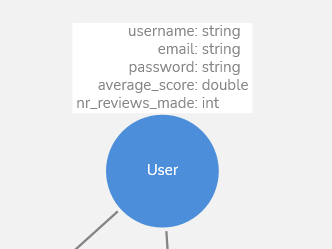
\includegraphics[]{exemplu_6_neo4j}
\caption*{}
\end{figure}

\begin{figure}[H]
\centering
\caption{Recenzia}
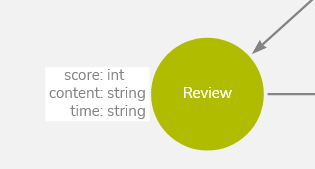
\includegraphics[]{exemplu_7_neo4j}
\caption*{}
\end{figure}

\begin{figure}[H]
\centering
\caption{Jocul}
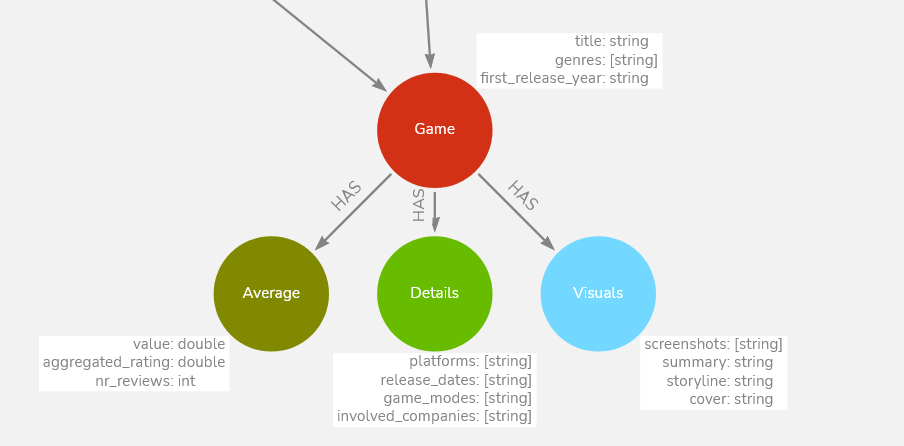
\includegraphics[scale = 0.6]{exemplu_8_neo4j}
\caption*{}
\end{figure}



\begin{figure}[H]
\centering
\caption{Schema bazei de date}
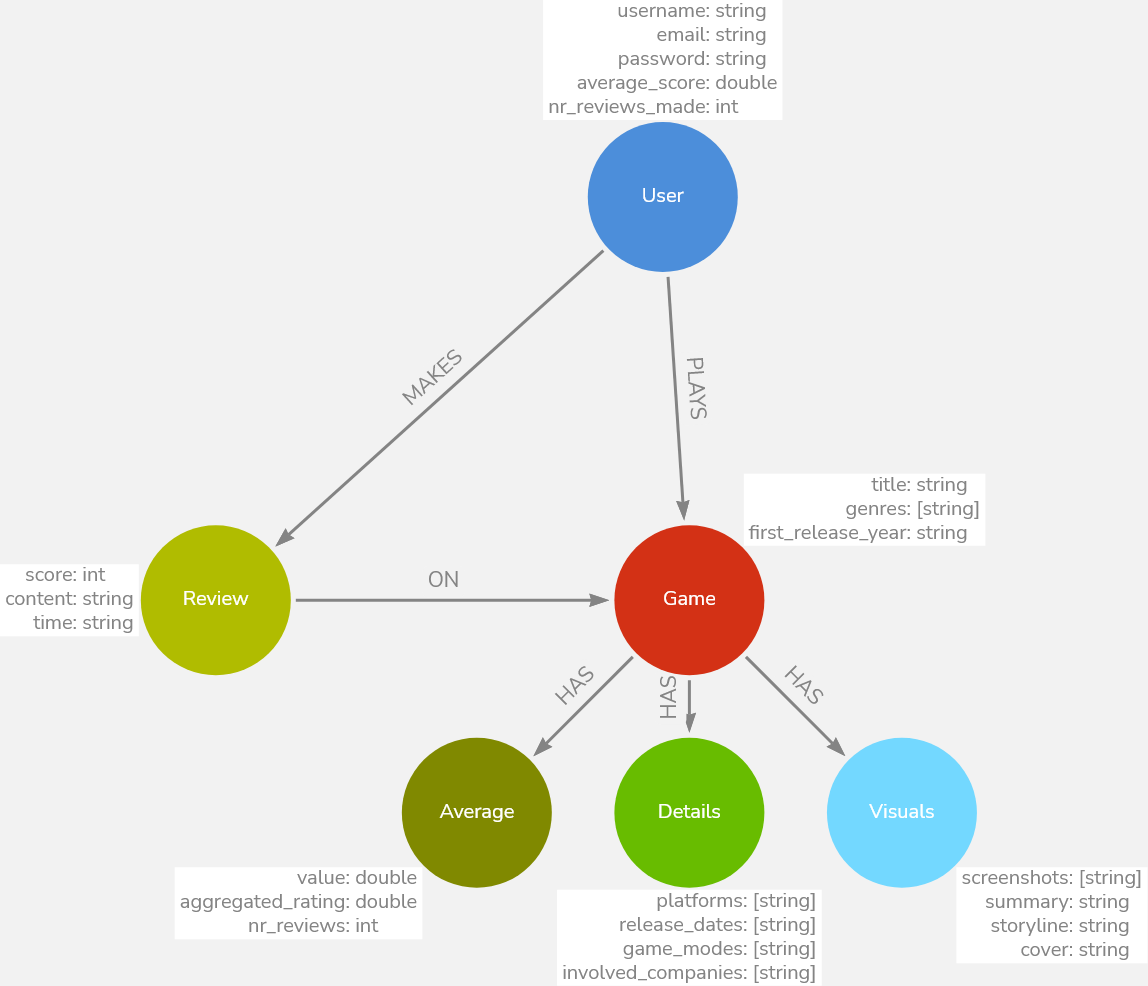
\includegraphics[scale=0.4]{exemplu_5_neo4j}
\caption*{Entitățile etichetate cu User, Game și Review mai au o proprietate în plus, și anume cea de id, care reprezintă un identificator unic pentru entitățile respective(uuid)}
\end{figure}

\subsection{Potențiale probleme}

\bigskip
\textbf{Constrângeri}
\bigskip

Am menționat atunci când am introdus capitolul de Baze de date faptul că două noduri care au aceeași etichetă nu trebuie să aibă neapărat aceleași proprietăți. Acest aspect face ca, în mod implicit, ca manipularea datelor să fie mult mai tolerabilă(cu mai puține constrângeri) în comparație cu o bază de date de tip SQL, unde acolo de exemplu trebuie să specificăm pentru o tabelă ce coloane să aibă și de ce tipuri să fie acestea.

Totuși, ce ar fi dacă am vrea să stabilim niște constrângeri? Poate am vrea să spunem de exemplu că o entitate etichetată cu User trebuie să aibă neapărat proprietățile \emph{username}, \emph{email} și \emph{password}, sau am vrea să setăm pentru o entitate cheia sa, ca să o putem identifica. Pentru a rezolva acest lucru, Neo4j introduce conceptul de constrângeri (\emph{constraints}) \cite{12}

Pentru a lucra facil cu baza noastră de date, Neo4j oferă o aplicație desktop ce vine cu un panou de comandă care oferă multe utilități. Putem executa de exemplu interogări în Cypher și să vizualizăm în mod interactiv graful obținut, cum se poate observa și în \textbf{Figura 4}.

În figura de mai jos, am realizat o captură în acest panou de comandă în care am scris comanda \texttt{SHOW CONSTRAINTS} unde pot vedea ce constrângeri sunt setate.

\begin{figure}[H]
\centering
\caption{}
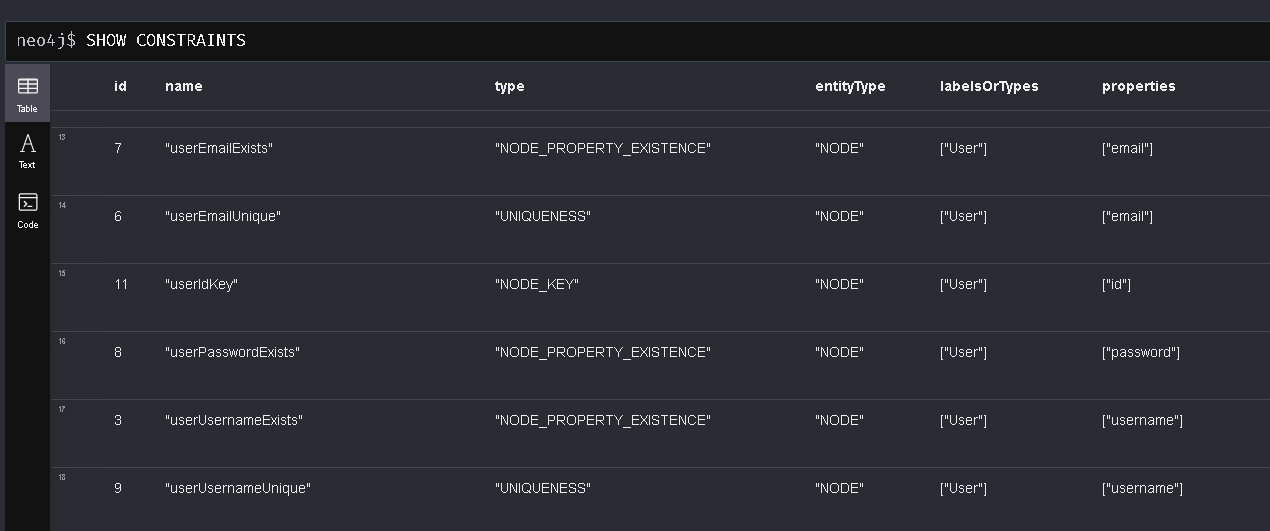
\includegraphics[scale = 0.5]{exemplu_9_neo4j}
\caption*{Se pot observa constrângerile pe care le-am setat pentru entitatea User}
\end{figure}

\bigskip
\textbf{Modul în care se actualizează scorul mediu al utilizatorului și al nodului \emph{Average} asociat nodului \emph{Game}}
\bigskip

Am menționat atunci când am prezentat schema bazei de date de faptul că am dori să ținem cont de scorul mediu al utilizatorului și al jocului, și de numărul de recenzii al acestor entități. O variantă naivă pentru a rezolva această problemă este să calculăm valorile acestor proprietăți în serverul de back-end, parcurgând toate recenziile asociate unui utilizator/joc și calculând media aritmetică a scorurilor acestora de fiecare dată când se face o nouă recenzie de exemplu. Dacă avem relativ puține date, nu ar fi o problemă, însă atunci când numărul de recenzii, de jocuri sau de utilizatori crește semnificativ, atunci trebuie abordată o altă soluție pentru a eficientiza acest proces.

Neo4j introduce un alt concept, prin intermediul librăriei APOC \cite{13}, cel de declanșatoare
(\emph{triggers}). \cite{14}
Declanșatoarele sunt folosite pentru a executa cod în Cypher înainte sau după ce anumite date au fost modificate.

Așadar, am putea folosi un declanșator pentru a actualiza numărul de recenzii și scorul mediu pentru entitățile \emph{User} și \emph{Game} după ce o recenzie a fost creată.

Pentru a înțelege codul ce va fi prezentat ulterior, voi introduce un mic artificiu matematic pentru a înțelege cum se actualizează media scorurilor în acest caz.

\bigskip

Să presupunem că după \( k \) recenzii efectuate, scorul mediu este \( a_k \) și cea de a \( k+1 \) recenzie are scorul \( s \).

Pentru a reconstitui suma anterioară, aceasta reprezintă pur și simplu produsul dintre \( k \) și \( a_k \). Așadar, putem calcula noua medie, prin formula: 

\[ a_{k+1} = \frac{k \cdot a_k + s}{k+1} \]

Prin urmare, fiind introdusă această formulă, se poate prezenta codul ce va fi executat în cadrul declanșatorului, în rândurile următoare:

\begin{figure}[h]
\centering
\begin{BVerbatim}
 UNWIND \$createdRelationships AS r 
    MATCH (review:Review)-[r:ON]->(game:Game)
    MATCH (game)-[:HAS]->(average:Average)
    MATCH (u:User)-[:MAKES]->(review)-[:ON]->(game)
    SET average.value = toFloat(
    average.nr_reviews * average.value + toInteger(review.score)
    ) / (average.nr_reviews + 1),
	average.nr_reviews = average.nr_reviews + 1,
    u.average_score = toFloat(
    u.nr_reviews_made * u.average_score + toInteger(review.score)
    ) / (u.nr_reviews_made + 1),
    u.nr_reviews_made = u.nr_reviews_made + 1
\end{BVerbatim}
\caption*{A se ignora simbolul \textbackslash{ } înainte de createdRelationships}
\end{figure}

Așadar, de fiecare dată după ce se creează o relație de tipul \texttt{ON} între nodurile \emph{Review} și \emph{Game}, atunci vom interoga nodurile \emph{Average} și \emph{User} pe care dorim să le actualizăm folosind formula anterioară.

\subsection{Generarea datelor de intrare}

Neo4j oferă funcționalitatea de a importa date prin intermediul fișierelor CSV, iar prin intermediul limbajului Cypher, pot fi create noduri și relații cu aceste date pentru a crea schema de baze de date.

Din intenția de a-mi modela baza de date după bunul meu plac, nu am vrut să optez pentru a lua un set de date deja gata făcut, ci am implementat un submodul în limbajul Java(separat de aplicația web propriu-zisă) care extrage date ori din API-uri externe(menționate la capitolul \textbf{Tehnologii și resurse folosite}, ori din fișiere salvate local, și generează fișiere CSV pentru a le putea importa apoi în baza de date.

\bigskip
\textbf{Generarea utilizatorilor}
\bigskip

Pentru a-mi genera utilizatorii fictivi ai aplicației, am apelat la librăria Java Faker. Aceasta m-a ajutat ca să generez nume de utilizator, parole și adrese de e-mail. În ceea ce privește parolele, am generat prin intermediul acestei librării un șir de caractere \emph{random} format din 8 caractere, ce conține cifre și litere. De asemenea, pe această parolă am aplicat o funcție hash, cu scopul de a nu fi stocată parola originală în baza de date, deci pentru a avea un strat de securitate în acest caz. Am ales să utilizez algoritmul PBKDF2 în convertirea parolei deoarece este o variantă sigură. \cite{15}

Așadar, cu valorile generate, am creat două fișiere CSV în care rețin 500 de utilizatori(un fișier cu parolele originale, celălalt cu parolele convertite prin funcția hash)

O observație importantă este că atât pentru utilizator, cât și pentru celelalte entități, am generat și un identificator unic, prin intermediul utilitarului UUID oferit de Java.

\bigskip
\textbf{Generarea jocurilor}
\bigskip

Pentru a-mi procura jocurile, m-am folosit de API-ul oferit de cătrei cei de la IGDB.

Pentru a putea utiliza acest API, a fost necesară crearea unui cont pe Twitch, iar prin intermediul acestui cont, mi-am generat un \emph{Client ID} și un \emph{Client Secret}. Cu aceste credențiale, am generat un \emph{token} pe care l-am folosit ca să pot accesa după API-ul menționat. Mai multe detalii pot fi regăsite aici. \cite{16}

În figura următoare, am atașat o bucată de cod prin care se poate observa cum utilizez acest API pentru a procura jocurile.

\begin{figure}[H]
\centering
\caption{}
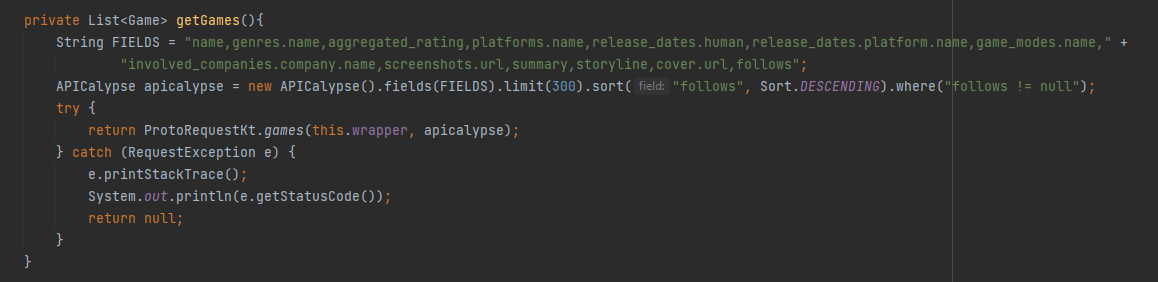
\includegraphics[scale = 0.6]{exemplu_10_games}
\caption*{Așadar, acele proprietăți enumerate în proprietatea FIELDS sunt practic cele folosite pentru modelarea entității \emph{Game} din baza de date. Am procurat 300 de jocuri pe care le-am sortat descrescător după proprietatea \emph{follows} pentru a mă asigura că voi lua cele mai populare jocuri cu putință. }
\end{figure}

După ce am obținut jocurile, am împărțit proprietățile așa cum am menționat la subcapitolul \textbf{Modelarea bazei de date} și am creat 4 fișiere CSV (games.csv, details.csv, visuals.csv, average.csv)

\bigskip
\textbf{Algoritmul lui Durstenfield}
\bigskip

Înainte de a trece la secțiunile următoare, am să prezint un algoritm care extrage în mod \emph{random} un număr de \( k\) elemente dintr-o listă cu scopul de a-l folosi în repartizarea jocurilor și a recenziilor cățre fiecare utilizator.

Acest algoritm a fost introdus de către Richard Durstenfield și este o variantă modernizată a aloritmului Fisher-Yates. \cite{16} Aceasta presupune parcurgerea listei(ori de la capăt, ori de la început) și schimbarea elementului curent cu un element ales în mod \emph{random}. Dacă toată lista este parcursă, atunci vom obține o permutare a listei inițiale.

Deoarece avem de extras \( k \) elemente din listă, atunci nu e nevoie să parcurgem toată lista, ci doar primele/ultimele \( k \) elemente. După aceste \( k \) schimbări, putem extrage elementele dorite, ori de la începutul, ori de la sfârșitul listei.

O variantă de implementare a algoritmului în limbajul Java ar putea arăta în felul următor:

\begin{figure}[H]
\centering
\caption{}
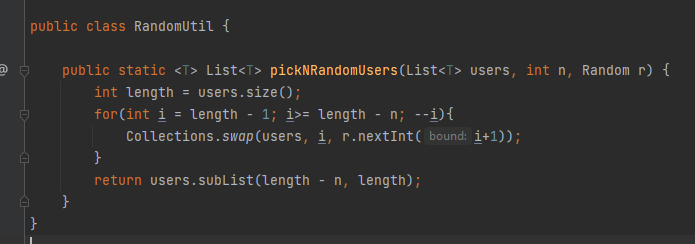
\includegraphics[scale = 0.8]{exemplu_11_random}
\caption*{Complexitatea acestui algoritm este \(\mathcal{O}(n) \), cu condiția ca metoda care alege în mod întâmplător elementul care trebuie schimbat să se facă în complexitate \(\mathcal{O}(1) \) }
\end{figure}

\bigskip
\textbf{Repartizarea jocurilor jucate către fiecare utilizator}
\bigskip

În această secțiune se poate observa deja utilitatea algoritmului menționat anterior. Pentru fiecare utilizator, am ales la întâmplare un număr de jocuri din cele 300 generate, iar aceste asocieri le-am salvat în fișierul plays.csv

Acest fișier arată în felul următor:

\begin{figure}[H]
\centering
\caption{}
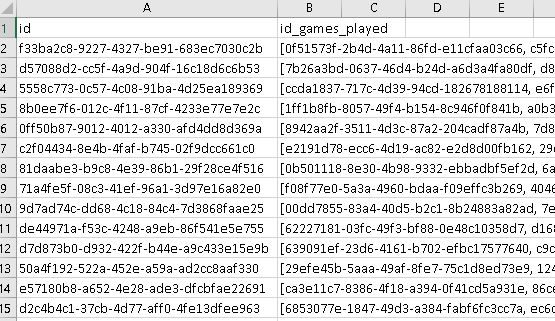
\includegraphics[scale = 0.8]{exemplu_12_plays}
\caption*{De menționat faptul că în coloana id\_games\_played sunt salvate niște liste de uuid-uri. În mod intuitiv, fișierele CSV generate ar putea fi asociate cu tabele dintr-o bază de date relațională. În acest caz, dacă am ignora faptul că id-urile jocurilor sunt reținute sub forma unei liste, am putea asocia conținutul fișierului plays.csv cu o tabelă asociativă. Practic aici se identifică o relație de mai mulți la mai mulți(un utilizator poate avea mai multe jocuri, iar un joc poate fi jucat de mai mulți utilizatori) }
\end{figure}

\bigskip
\textbf{Generarea recenziilor și repartizarea acestora către fiecare utilizator}
\bigskip

În această secțiune, am folosit atât API-ul oferit de Steam pentru a obține recenziile unui joc, dar și fișiere salvate local pentru a încerca să optimizez cât mai mult timpul necesar pentru a fi generate toate fișierele.

Primul pas a fost să salvez într-un fișier local în format JSON jocurile oferite de Steam, sub forma unei liste de obiecte, în care fiecare obiect are două proprietăți:  \emph{appid}(un identificator unic folosit de Steam pentru jocurile sale) și \emph{name}(numele jocului). Scopul acestui fișier este de a încerca să identific dacă jocul procurat inițial de la IGDB API poate fi identificat ca un joc din platforma Steam ca să pot extrage ulterior recenzii relevante acestui joc. (prin intermediul API-ului oferit de Steam). În caz contrar, voi extrage o recenzie aleatoare dintr-un fișier salvat local de tip csv dintr-un set de date oferit de Kaggle. \cite{17}

Al doilea pas a fost să asociez fiecărui utilizator un număr de recenzii pe care le poate oferi din acele jocuri pe care le-am repartizat. Acest număr de recenzii a fost deasemenea generat la întâmplare.

După ce am determinat acest număr, voi extrage acele jocuri ce urmează a fi recenzate, după care voi încerca să asociez pentru fiecare joc câte o recenzie. 

Pentru a fi mai ușor de explicat, următorii pași îi voi ilustra sub forma unui pseudocod, iar după acest pseudocod va fi prezentat codul propriu-zis în Java, pentru a fi mai ușor de înțeles.

\begin{figure}[H]
\centering
\caption{}
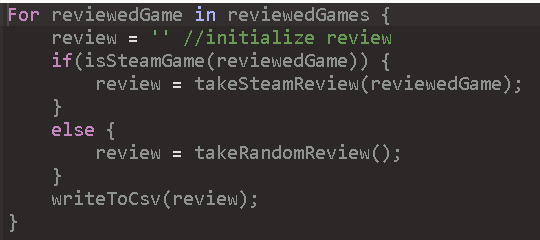
\includegraphics[scale = 0.8]{exemplu_13_review_code}
\caption*{La o primă vedere, acest procedeu nu este complicat, însă dificultatea constă în extragerea unei recenzii pentru un joc aflat pe platforma Steam, deoarece trebuie gestionată frecvența \emph{request}-urilor care se fac către API-ul care ne oferă recenziile în acest caz. De menționat faptul că acest procedeu se realizează pentru fiecare utilizator.}
\end{figure}

O modalitate naivă este de a face un \emph{request} de fiecare dată când dorim să asociem o recenzie unui joc, însă numărul de \emph{request-uri} crește cu cât mărim numărul de utilizatori și de jocuri recenzate de fiecare utilizator. În cazul de față, avem \(500\) de utilizatori, și să presupunem că pentru fiecare utilizator avem în medie \(20\) de recenzii, deci în total \(10 000 \) de \emph{request}-uri.

Să presupunem că timpul mediu în care s-ar face un request este de \( 20 \) milisecunde.(un timp foarte bun în practică) În total ar dura \( 10 000 \cdot 20 = 200000 \approx 3 \) minute, ceea ce este un timp deloc neglijabil în acest context.

O observație importantă este faptul că un joc căruia i se extrage o recenzie este foarte posibil să se repete atunci când se parcurg utilizatorii. De asemenea, nu suntem constrânși de către API să extragem fix o recenzie, putem extrage mai multe dacă se dorește acest lucru, ceea ce sporește varietatea recenziilor pentru același joc, în cazul în care se repetă.

O structură de date folositoare oferită de limbajul Java pentru a fructifica acest aspect este cea numită \emph{Map}, în care se rețin perechi tip cheie-valoare. În contextul nostru, cheia este un joc, iar valoarea este reprezentată de recenziile jocului, sub forma unui JSON. Inițializarea acestuia ar putea arăta în felul următor:

\begin{verbatim}
  private final Map<SteamGame, JsonNode> reviewsRegistry = new HashMap<>();
\end{verbatim}

Așadar, dacă jocul există deja în această structură de date, atunci voi extrage o recenzie deja stocată. În caz contrar, voi face un \emph{request} pentru a obține recenziile.

Codul implementat în Java arată în felul următor:

\begin{figure}[H]
\centering
\caption{}
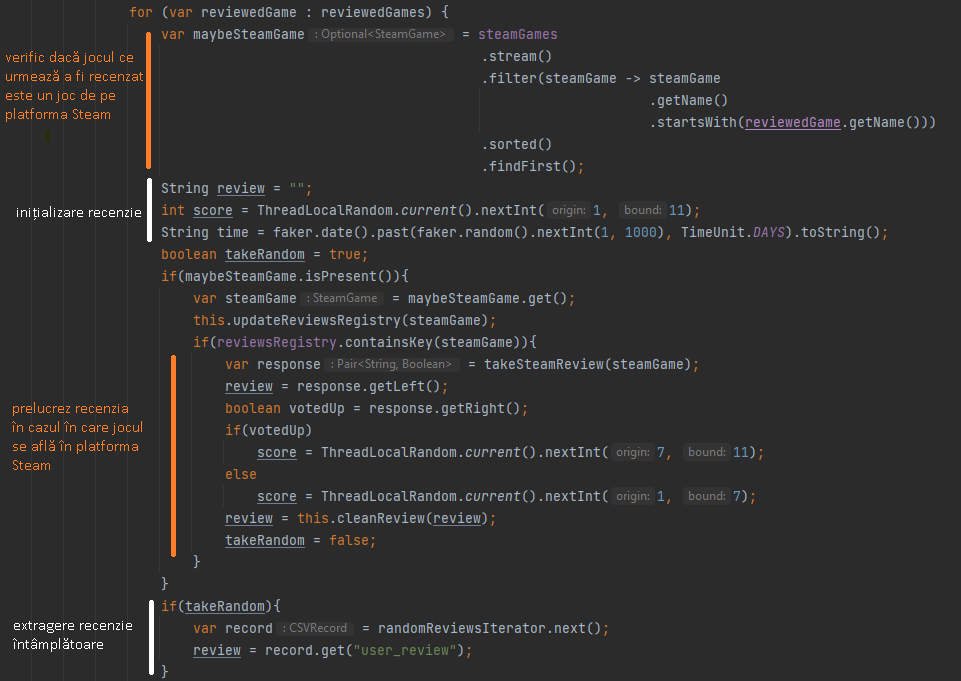
\includegraphics[scale = 0.7]{exemplu_14_review_code_java}
\caption*{Se poate observa folosirea proprietății \emph{votedUp}, pusă la dispoziție de către API-ul responsabil de recenzii de la Steam, prin care verific dacă acea recenzie a fost pozitivă sau negativă. În funcție de acest verdict, încerc să generez un scor care să reflecte cât mai mult realitatea.}
\end{figure}

Așadar, acesta este submodulul care se ocupă de generarea fișierelor CSV necesare pentru a putea importa conținutul acestora în baza de date.

\subsection{Importarea conținutului fișierelor CSV în baza de date}

Modul prin care sunt importate aceste date este prin intermediul limbajului Cypher, mai concret prin comanda \texttt{LOAD CSV} ce face parte din acest limbaj \cite{18}.

Un exemplu de cod în Cypher în care îmi creez recenziile generate poate fi acesta:

\begin{figure}[H]
\centering
\begin{BVerbatim}
LOAD CSV WITH HEADERS
FROM 'file:///reviews.csv'
AS line
MATCH(u:User {id: line.id_user})
MATCH(g:Game {id: line.id_game})
MERGE(r:Review {id: line.id_review})
    ON CREATE SET r.score = line.score,
                  r.content = line.content,
                  r.time = line.time
MERGE (u)-[:MAKES]->(r)-[:ON]->(g)
\end{BVerbatim}
\caption*{Un element de noutate este reprezentat de clauza \texttt{MERGE}. Prin aceasta putem verifica, în acest caz, dacă nodul \emph{Review} a fost creat sau există deja. În cazul în care este creat, atunci vor fi setate proprietățile aferente. În cazul în care acest cod ar fi rulat a doua oară(fără alte modificări în prealabil), atunci nu va fi creat niciun nod nou, deci practic nu va mai avea niciun efact.}
\end{figure}

De-a lungul timpului cât am dezvoltat acest submodul de generare a fișierelor CSV, am întâmpinat uneori dificultăți care au făcut necesare ștergerea datelor din baza de date și reintroducerea acestora cu modificările aferente. Pentru a ușura acest proces, Neo4j oferă prin intermediul panoului de comandă o secțiune prin care se pot marca coduri în Cypher ca favorite și pot fi executate ori de câte ori este nevoie.

Practic, mi-am salvat o serie de coduri în secțiunea de favorite pe care le pot executa în ordine atunci când este nevoie. 

\begin{figure}[H]
\centering
\caption{}
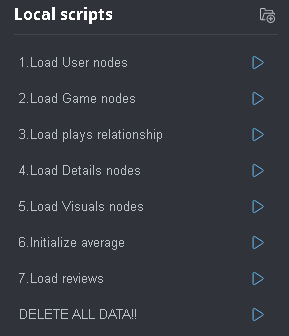
\includegraphics[scale = 0.8]{exemplu_15_favorites}
\caption*{}
\end{figure}

În ceea ce privește ștergerea întregului conținut al bazei de date, aceasta trebuie făcută cu grijă. Neo4j recomandă mai multe alternative prin care acest procedeu poate fi făcut utilizându-se cele mai bune practici, pentru a evita efecte secundare neplăcute. \cite{19}

Varianta pentru care am optat este următoarea:

\begin{figure}[H]
\centering
\begin{BVerbatim}
CALL apoc.periodic.iterate(
"MATCH (n) return id(n) as id",
"MATCH (n) WHERE id(n) = id DETACH DELETE n", 
{batchSize: 10000}
)
YIELD batches, total RETURN batches, total
\end{BVerbatim}
\caption*{Practic, prin intermediul librăriei APOC, șterg toate nodurile(cu tot cu relațiile asociate) în grupuri de câte 10000 de noduri.}
\end{figure}

După ce am importat datele, putem interacționa cu acestea prin intermediul panoului de comandă ca să se poată verifica dacă datele au fost întradevăr, introduse corect.

Una din modalitățile interesante prin care putem verifica asta este dacă schema bazei de date care a fost descrisă în subcapitolul \textbf{4.3 Modelarea bazei de date } se potrivește cu cea pe care o putem vizualiza în mod interactiv prin intermediul comenzii \texttt{CALL db.schema.visualization()}

Rezultatul acestei comenzi este reprezentat în figura de mai jos:

\begin{figure}[H]
\centering
\caption{}
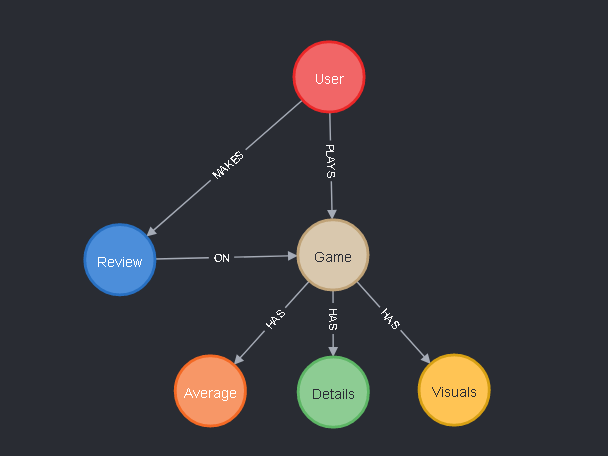
\includegraphics[scale = 0.7]{exemplu_16_schema}
\caption*{}
\end{figure}



\section{Back-end}

\subsection{De ce Java? De ce Spring Boot?}

Soluția aleasă pentru a stoca datele este una relativ de nișă, având în vedere caracteristica de NoSql a bazei de date Neo4j, dar și de faptul că are la bază o reprezentare de tip graf. Așadar, studiind soluțile oferite din această documentație \cite{20} legată de limbajele suportate de Neo4j, am observat că Java este singurul limbaj în care Neo4j oferă capabilitatea de a mapa nodurile ce se regăsesc în baza de date în entități, ceea ce oferă un mod de lucru facil cu o perspectivă de ansamblu mult mai mare, în comparație cu un \emph{driver} în care modul de lucru este unul mult mai elaborat. Această soluție se numește \emph{Spring Data Neo4j}. \cite{21}

Având în vedere faptul că capabilitățile de a lucra mult mai facil cu baza de date se regăsesc în suita Spring, am ales să utilizez Spring Boot pentru a implementa serverul de back-end. Faptul că am avut o introducere în acest \emph{framework} în cadrul materiei \emph{Programare avansată} din anul 2 semestrul 2 de studiu mi-a dat un punct de pornire consistent pentru a dezvolta această parte de back-end.


\subsection{Modelarea nodurilor în entități}

Așa cum am menționat la introducerea acestui capitol, soluția folosită pentru a mapa nodurile în entități este cea oferită de \emph{Spring Data Neo4j}.

Această mapare presupune reprezentarea nodurilor din schema bazei de date (\emph{User}, \emph{Review} și \emph{Game}) sub forma unor clase(entități) care pot fi utilizate pe partea de back-end. O instanță a acestei clase reprezintă practic un nod din baza de date.

La baza acestor mapări stau adnotările, iar cele care au fost utilizate în cadrul aplicației în mod frecvent sunt: \emph{@Id}, \emph{@Property}, \emph{@Relationship}. Pentru a explica utilizarea lor, va fi reprezentată următoarea figură:

\begin{figure}[H]
\centering
\caption{}
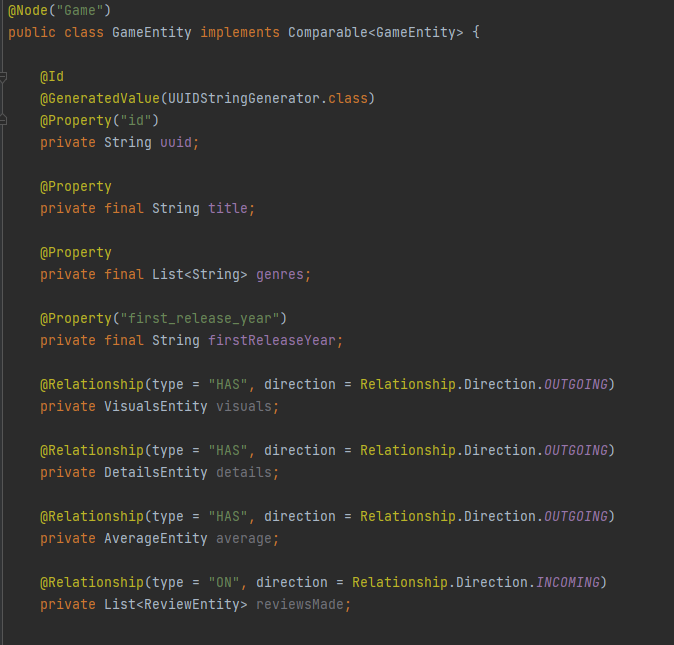
\includegraphics[scale = 0.8]{exemplu_18_adnotari}
\caption*{Entitatea \emph{Game}}
\end{figure}

În primul rând, se observă adnotarea clasei \emph{GameEntity} cu \emph{@Node("Game")}, care asociază reprezentarea acestei clase cu cea a nodului din schema bazei de date etichetat cu "Game".

Cu adnotarea \emph{@Id} se specifică proprietatea care identifică în mod unic o entitate. Având în vedere faptul că se utilizează \emph{uuid}-uri, adnotarea \emph{@GeneratedValue} ajută la specificarea unui generator care face în mod automat un \emph{uuid}, un aspect util atunci când se instanțiază o nouă entitate, de exemplu.

Adnotarea \emph{@Property} este utilă pentru a asocia proprietățile corespunzătoare nodurilor din schema bazei de date cu proprietățile din această clasă.(e.g. proprietățile \emph{title}, \emph{genres}, \emph{firstReleaseYear})

Adnotarea \emph{@Relationship} este utilă atunci când se dorește ținerea în evidență a relațiilor pe care le poate avea entitatea definită cu celelalte entități. În acest caz, cum nodul \emph{Game} are cele trei noduri \emph{Visuals}, \emph{Details} și \emph{Average} care îl extind pe acesta, se poate observa în mod intuitiv utilizarea acestei adnotări. O relație este definită prin intermediul unui tip și al unei direcții("înspre" entitatea definită, sau "în afara" entității.) De asemenea, se observă ținerea în evidență a recenziilor care s-au făcut asupra jocului.

O observație importantă în ceea ce privește încărcarea datelor asociate unei relații, este faptul că aceasta se face doar atunci când este în mod explicit nevoie. De exemplu, dacă am dori să obținem o entitate \emph{GameEntity} în funcție de \emph{uuid}, atunci datele obținute sunt doar cele aferente proprietăților(adică nu se vor încărca datele asociate nodurilor \emph{Visuals}, \emph{Details} și \emph{Average}) pentru un plus de performanță.

Pentru a avea mai mult control asupra datelor ce se doresc a fi obținute, va fi prezentată secțiunea următoare.

\subsection{Interfața Repository și conceptul de Interface Projection}

Scopul interfeței Repository este de a oferi un mod abstract și facil prin intermediul căruia este implementat un strat de acces care poate fi utilizat pentru a reduce în mod semnificativ codul implementat în interacționarea cu datele. \cite{22}

Această interfață este definită în mod generic, luând doi parametrii: numele entității care va fi prelucrată și tipul de date al identificatorului(în cazul de față \emph{String})

Metodele specifice acestei interfețe fac parte din repertoriul CRUD(Create, Read, Update, Delete.)

Un exemplu de definire a acestei entități poate fi observat în figura următoare:

\begin{figure}[H]
\centering
\caption{}
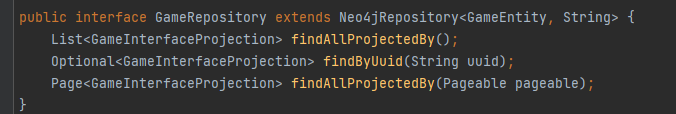
\includegraphics[scale = 0.8]{exemplu_19_repository}
\caption*{Interfața de tip \emph{Neo4jRepository} specifică entității \emph{GameEntity}}
\end{figure}

În mod convențional, metodele sunt numite astfel încât să se poată observa tipul operației, folosindu-se cuvinte cheie precum \emph{find}, \emph{by}, \emph{save}, iar implementarea acestora se face în mod automat la \emph{runtime}. În exemplul din figură, metodele sunt de tipul Read: una pentru a obține toate jocurile stocate, una pentru a obține un joc după un \emph{uuid}, și una pentru a obține jocurile prin intermediul paginării(de exemplu: o pagină de 5 jocuri)

Se oferă suport și pentru definirea unor metode \emph{custom} în cazul în care este nevoie de obținerea unui rezultat în urma unei interogări în limbajul \emph{Cypher}, însă mai multe detalii legat de acest aspect se pot regăsi în capitolul 6 \textbf{Algoritmul de recomandare}.

De asemenea, se poate observa apariția conceptului de \emph{Interface Projection}, prin care se poate preciza prin intermediul unei interfețe ce date să fie prelucrate dintr-o entitate. 

În cazul de față, să presupunem că dorim să avem pentru entiatea \emph{GameEntity} și acele date care extind nodul \emph{Game} aferent din baza de date (\emph{Visuals}, \emph{Details} și \emph{Average}). Așadar, putem să ne definim o interfață(de exemplu cu numele de \emph{GameInterfaceProjection}) care precizează datele de care avem nevoie. Aceasta arată în felul următor:

\begin{figure}[H]
\centering
\caption{}
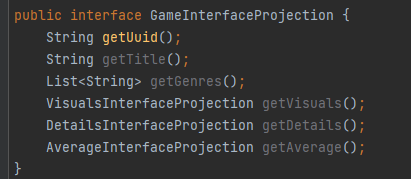
\includegraphics[scale = 1]{exemplu_20_interface_projection}
\caption*{Un lucru interesant de menționat este faptul că aceste proiecții pot fi definite în mod recursiv. În cazul de față, \emph{Visuals}, \emph{Details} și \emph{Average} sunt de asemenea entități, și datele acestora pot fi controlate separat prin intermediul unui \emph{Interface Projection} specific.}
\end{figure}


\subsection{REST API}

Modul prin care funcționalitățile de pe back-end sunt expuse spre a fi folosite de către serverul de front-end este prin intermediul unui REST API, în care resursele oferite sunt reprezentate sub format JSON.

Expunerea acestor funcționalități s-a făcut prin intermediul \emph{Controller}-elor: \emph{UserController}, \emph{GameController} și \emph{ReviewController}. Acestea utilizează în mod intern servicii implementate care se utilizează de metodele din \emph{repository}. De exemplu, se poate regăsi în figura de mai jos modul cum a fost definit \emph{ReviewController}:

\begin{figure}[H]
\centering
\caption{}
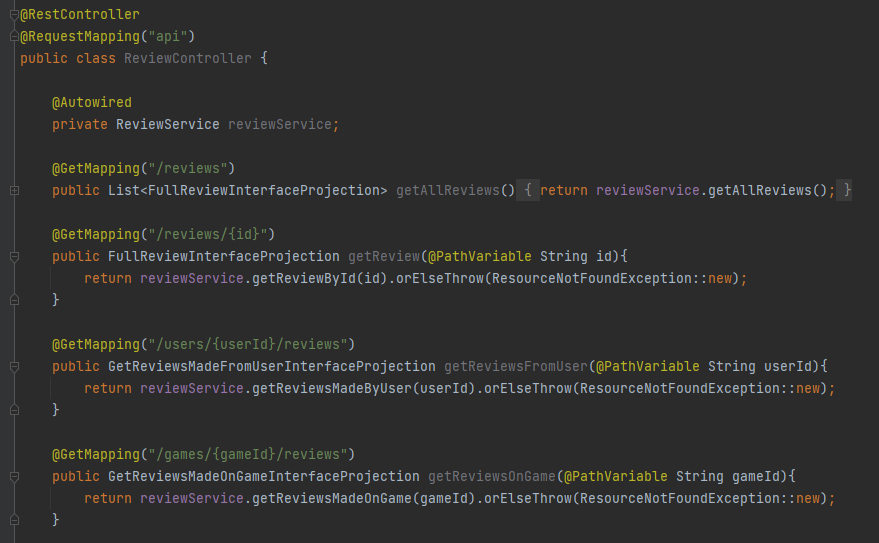
\includegraphics[scale = 0.7]{exemplu_21_review_controller}
\caption*{}
\end{figure}

Adnotările sunt și în acest caz destul de sugestive. Practic, sunt definite mai multe \emph{request-uri} de tipul GET ce pot fi accesate prin intermediul protocolului HTTP. Acestea au rolul de a oferi resurse(recenzii), mai concret ori toate recenziile disponibile, ori o recenzie în funcție de id, ori toate recenziile făcute de un utilizator, ori toate recenziile făcute asupra unui joc.

Adnotarea \emph{@Autowired} denotă faptul că instanța serviciului \emph{ReviewService} este injectată spre a fi folosită în acest controller. Acest aspect ilustrează conceptul de \emph{Dependency Injection}, care are ca scop reducerea cuplării. \cite{23}

Acest serviciu este responsabil de procurarea datelor necesare prin intermediul \emph{repository-urilor} definite.

Modul cum a fost implementat se regăsește în următoarea figură:

\begin{figure}[H]
\centering
\caption{}
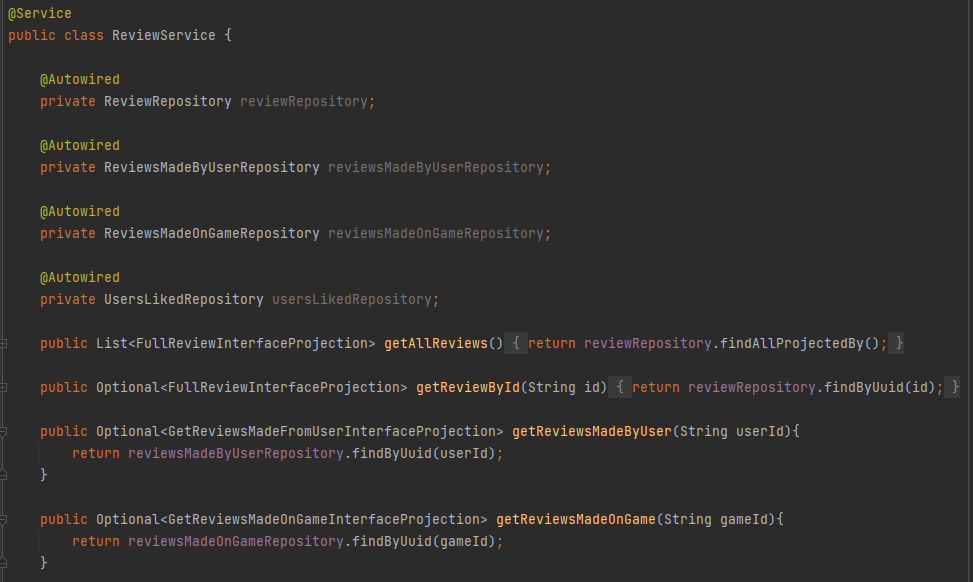
\includegraphics[scale = 0.65]{exemplu_22_review_service}
\caption*{}
\end{figure}

Se poate observa că implementarea propriu-zisă este aproape trivială în acest caz. Totuși, o implementare netrivială se poate regăsi în capitolul 6 \textbf{Algoritmul de recomandare}.





\subsection{Modulul de autentificare al utilizatorilor}


   Acest modul are un scop relativ simplu, fiind reprezentat de valorificarea fișierului csv în care sunt reținute parolele convertite de funcția hash, dar și de a persista starea de logare a utilizatorului pe partea de front-end a aplicației, prin intermediul unui JWT token. \cite{24}

Implementarea acestuia reprezintă doar un punct de pornire, căci poate fi extins și prin introducerea autorizării, în care anumite \emph{request-uri} din API pot fi autorizate în funcție de rolul pe care îl are utilizatorul prin intermediul token-ului menționat anterior. Totuși, pentru scopul în mare al proiectului, acela de a observa cum se poate rezolva problema recomandării unor jocuri video, acest aspect de autentificare/autorizare nu a fost atins foarte în detaliu.

Pentru a implementa acest modul, am utilizat funcționalitățile oferite de \emph{Spring Security}. \cite{25}

În general, o aplicație web Spring are la bază un \emph{Dispatcher Servlet}, care, în mod intuitiv conform numelui, acționează ca un dispecer care verifică ce \emph{request} s-a făcut și îl asociază cu unul definit în cadrul unui metode din \emph{Controller}. \cite{26}

Totuși, nu am menționat niciun aspect legat de securitate, iar de acest lucru se ocupă \emph{Spring Security}, care în linii mari include posibilitatea de a adăuga unul sau mai multe filtre înainte de a acționa acel \emph{Dispatcher Servlet}.

Pentru a stabili aceste filtre, am suprascris anumite metode din cadrul clasei abstracte \emph{WebSecurityConfigurerAdapter} în clasa numită \emph{WebSecurityConfig} în felul următor:

\begin{figure}[H]
\centering
\caption{}
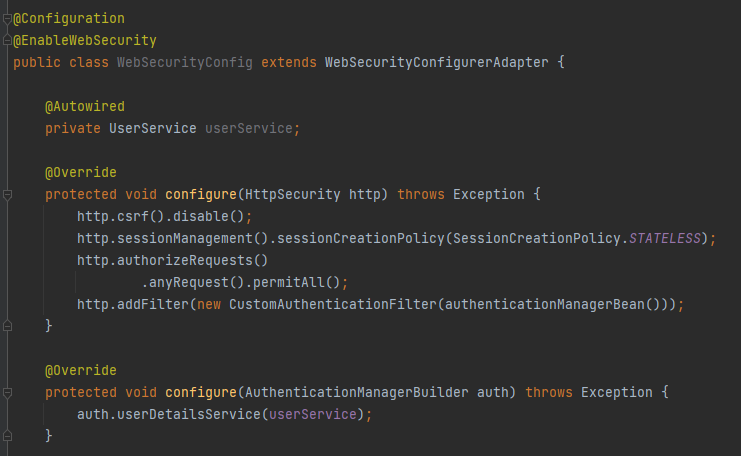
\includegraphics[scale = 0.7]{exemplu_23_security}
\caption*{}
\end{figure}

În stadiul actual, practic orice \emph{request} are cale liberă spre a fi folosit, însă acest lucru poate fi bineînțeles schimbat ulterior prin autorizarea \emph{request}-urilor în funcție de rolurile utilizatorului.

De asemenea, a fost implementat un \emph{userService} care are rolul de a prelua un utilizator după \emph{username}-ul său.

Punctul de interes îl reprezintă acel \emph{CustomAuthenticationFilter} care prelucrează credențialele
(numele de utilizator și parola) din cadrul \emph{request}-ului care se ocupă de autentificarea unui utilizator, și acționează corespunzător dacă autentificarea s-a efectuat cu succes sau nu. În caz pozitiv, acest \emph{request} va furniza un JWT token ce va fi folosit de către aplicația de front-end pentru a persista logarea utilizatorului.

O variantă de implementare concretă a furnizării acelui \emph{token} poate fi următoarea:


\begin{figure}[H]
\centering
\caption{}
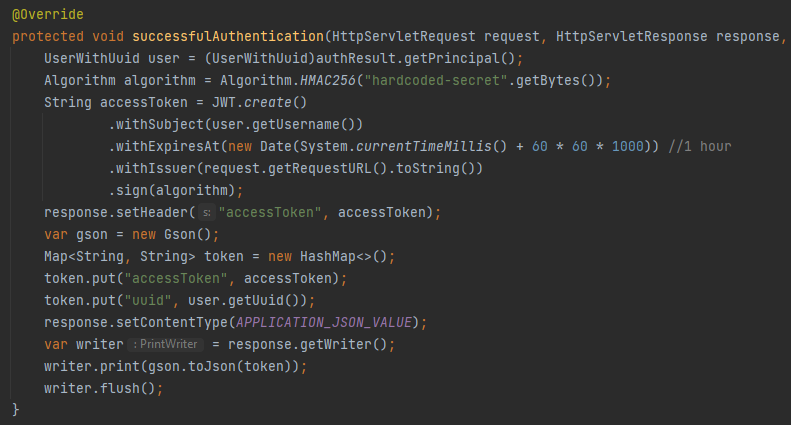
\includegraphics[scale = 0.75]{exemplu_24_jwt}
\caption*{}
\end{figure}

De menționat faptul că acel secret care este pus manual pentru a fi folosit în semnarea \emph{token}-ului prin intermediul algoritmului HMAC nu este o metodă bună în practică(în contextul unei eventuale lansări ipotetice a aplicației în producție), însă în scopul de față, acest aspect nu reprezintă un inconvenient major.


\newpage



\section{Algoritmul de recomandare}

Documentația pe care am consultat-o în scopul implementării acestui algoritm constă într-un curs de pe Udemy. \cite{27} Chiar dacă în acest curs noțiunile sunt prezentate având ca limbaj suport Python, intenția mea a fost de a înțelege mai degrabă conceptele și de a le implementa utilizând limbajul Java și baza de date Neo4j.

\subsection{Introducere}

Se observă o tendință ascendentă în ultimii 20-30 de ani în ceea ce privește atât conținutul informațiilor ce se regăsește pe internet, cât și numărul utilizatorilor acesteia. \cite{28} Așadar, se pune problema de a filtra cât mai eficient aceste informații pentru ca utilizatorul să obțină ceea ce își dorește. O modalitate este reprezentată de folosirea unor motoare de căutare, cel mai cunoscut fiind cel de la \emph{Google}. \cite{5}

Totuși, acest lucru nu garantează în mod implicit identificarea unor informații care să fie personalizate în funcție de interesele utilizatorului. Un exemplu clasic ar fi reprezentat de un magazin online, în care utilizatorul, în funcție de anumite caracteristici, precum istoricul comenzilor sale, recenziile pe care le-a făcut la produse sau ultimele produse accesate, să poată primi recomandări de noi produse pe care, în cazul fericit, să le comande. Așadar, se încearcă găsirea unei soluții care practic să prezică unui utilizator viitoarele produse pe care ar dori să le comande în acest caz.

Această soluție este reprezentată de un sistem de recomandări.

\subsection{Categorii de sisteme de recomandări}

Un sistem de recomandări poate fi catalogat în două mari categorii:

\begin{enumerate}
  \item Sistem de recomandări bazate pe conținut
  \item Sistem de recomandări bazate pe filtrare colaborativă
\end{enumerate}

Sistemele de recomandări bazate pe \textbf{conținut} pun mai mult accent pe metadatele asociate unei resurse. Cu cât resursa ce se dorește a fi recomandată poate fi cât mai bine descrisă din acest punct de vedere, cu atât șansele de reușită ale unui algoritm care se încadrează în această categorie sunt mai mari. 

În schimb, sistemele de recomandări bazate pe \textbf{filtrare colaborativă} sunt pretate acelor resurse care nu pot fi desscrise cu ușurință prin intermediul metadatelor. În linii mari, algoritmii care se încadrează în acest sistem țin cont de recenziile altor utilizatori similari cu utilizatorul căruia i se furnizează o recomandare.

În secțiunea următoare, va fi descrisă soluția implementată în cadrul acestei aplicații, și anume un algoritm de recomandare bazat pe filtrare colaborativă.

\subsection{Recomandări bazate pe filtrare colaborativă}


   Înainte de a fi explicat algoritmul propriu-zis, vor fi introduse notații care vor facilita prezentarea algoritmului. 

\bigskip
\bigskip

Fie \( S \) un sistem de recomandare.

Fie \( n \) numărul de utilizatori existenți în cadrul sistemului \(S \).

Fie \( m \) numărul de resurse(jocuri)\footnote{teoretic, termenul de \emph{resurse} sau \emph{jocuri} poate fi folosit în mod interschimbabil, căci nu contează în mod specific ce resursă urmează a fi recomandată. Pentru simplitate, mă voi referi de acum încolo la termenul de \emph{jocuri}.}
 în cadrul sistemului \( S \).

\bigskip
\bigskip

\noindent Fiecare utilizator poate atribui un scor jocurilor. O modalitate prin care putem reprezenta acest fenomen este prin intermediul unei matrici care poate fi descrisă în felul următor:

\bigskip
\bigskip

Fie \( r_{ij} =  \) scorul pe care utilizatorul \( i \) îl atribuie jocului \( j \),

unde \( i = \overline{\rm 1,n} \), \( j = \overline{\rm 1,m} \)

\( R_{n \times m} = \) matrice de dimensiune \( n \times m\) în care sunt reținute scorurile pe care utilizatorii le pot da jocurilor.

\bigskip
\bigskip


\noindent În practică, această matrice este rară, adică sunt relativ puține elemente care să fie nenule. O observație importantă este faptul că dacă un utilizator atribuie unui joc scorul 0, asta nu înseamnă că acel element este considerat lipsă(gol), ci că utilizatorul a atribuit unui joc cel mai mic scor posibil. Așadar, matricea este rară nu din cauză că majoritatea elementelor au scorul 0, ci că la majoritatea utilizatorul \( i \) nu a atribuit un scor jocului \( j \).

La prima vedere, acest lucru nu ar putea fi considerat unul benefic, însă să presupunem următorul studiu de caz:

\bigskip

Fie platforma de jocuri video pentru PC numită Steam. În momentul scrierii acestei lucrări, există aproximativ \( 50 000 \) jocuri pe această platformă. \cite{29} Nu am găsit un număr concret legat de câți utilizatori ar exista, însă estimativ în jur de 60 de milioane de utilizatori folosesc Steam zilnic, și sunt 120 de milioane de utilizatori activi într-o lună, așadar, numărul este considerabil mai mare. Este cert mult mai mare decât numărul de jocuri existente.

În mod intuitiv, matricea asociată este una rară. Ca să explic mai bine această intuiție, am încercat să găsesc statistici legate de numărul de jocuri în medie deținute de un utilizator. Neoficial, un utilizator deține în jur de 11 jocuri. Acest aspect este îndeajuns pentru a motiva faptul că matricea este întradevăr rară.

Dacă matricea ar fi plină, atunci înseamnă practic că utilizatorii în mare au oferit recenzii majorității jocurilor existente, ceea ce înseamnă că nu se mai observă rostul de a oferi recomandări, de vreme ce matricea este plină. Așadar, este un lucru benefic faptul că matricea este rară, căci aceasta este problema pe care o încearcă un sistem de recomandări să o rezolve: să prezică scoruri pentru elementele lipsă din matrice.

\bigskip

Fie \( s(i, j) \) scorul ce se încearcă a fi prezis pe care utilizatorul \( i \) îl atribuie jocului \( j \).

\noindent O primă tentativă de a stabili o formulă pentru a calcula acest scor ar fi următoarea:

\[ s(i, j) = \dfrac{ \sum\limits_{i' \epsilon \Omega_{j} } r_{i'j} }{|\Omega_{j}|}\]

unde \( \Omega_{j}\) reprezintă mulțimea utilizatorilor care au atribuit un scor jocului \( j \).

\bigskip

Această formulă reprezintă defapt calcularea unui scor mediu, iar inconvenientul pe care îl prezintă este faptul că tratează fiecare utilizator în mod egal. Totuși, raportându-ne la un utilizator, există alți utilizatori care ar putea avea preferințe similare, și alți utilizatori care ar putea avea mai puține preferințe similare cu acesta.

Pentru a putea ajusta această formulă, o putem transforma într-o medie aritmetică ponderată, care arată în felul următor:

\[ s(i, j) = \dfrac{ \sum\limits_{i' \epsilon \Omega_{j} } w_{ii'} \cdot r_{i'j} }{\sum\limits_{i' \epsilon \Omega_{j}} w_{ii'}}  \]

În mod intuitiv, o pondere \( w_{ii'}\) arată cât de similar este utilizatorul \( i \) cu \(i'\). Adică, această pondere este cu atât mai mare cu cât \( i \) și \( i' \) au preferințe similare, și cu atât mai mică cu cât \( i \) și \( i' \) au preferințe mai puțin similare. Modul cum se poate calcula această pondere va fi descris ulterior.

Următorul exemplu va fi ilustrat cu scopul de a înțelege mai bine această intuiție:

\begin{center}
\begin{tabular}{||c c c c c c||} 
 \hline
 & DOOM Eternal & Battlefield & Call of Duty & The Witcher 3: Wild Hunt & Dark Souls III \\ [0.5ex] 
 \hline\hline
 Ion & 9 & 8 & 10 & 3 & 6 \\ 
 \hline
 Gigel & 8 & 9 & & 4 & 5  \\
 \hline
 Alex & 5 & 7 & 4 & 10 & 9 \\
 \hline
\end{tabular}
\end{center}

Se observă o matrice de scoruri cu trei utilizatori și 5 jocuri. Jocurile DOOM Eternal, Battlefield și Call of Duty sunt jocuri \emph{shooter}, în timp ce celelalte două jocuri sunt de gen \emph{RPG}(Role-playing game).

Din modul cum sunt distribuite scorurile, Ion preferă mai mult jocurile de tip \emph{shooter} în comparație cu jocurile de tip \emph{RPG}, în timp ce Alex preferă mai mult The Witcher 3 și Dark Souls III.

Gigel încă nu a atribuit un scor jocului Call of Duty, însă în mod intuitiv, am putea prezice faptul că valoarea scorului va fi destul de mare(este foarte probabil ca lui Gigel să-i placă Call Of Duty), căci se observă faptul că Gigel și Ion au preferințe similare. Așadar, ponderea între Ion și Gigel ar fi una relativ mare, iar cea între Alex și Gigel ar fi una relativ mică.

\newpage

Totuși, chiar și această medie aritmetică ponderată are un dezavantaj care este reprezentat de faptul că utilizatorii ar putea fi optimiști sau pesimiști în ceea ce privește scorurile pe care le atribuie jocurilor. 

De exemplu, un utilizator ar putea fi descris drept optimist dacă majoritatea scorurilor pe care le dă sunt note mari(9 sau 10), iar un utilizator pesimist este cel care oferă jocurilor în general scoruri mici(note între 1-5).

Pentru a putea exprima acest lucru, se introduce conceptul de \textbf{deviație}. În mod intuitiv, poate fi explicată astfel:

\bigskip

Dacă un utilizator este pesimist(are un scor mediu de 6) și oferă unui joc scorul 9, înseamnă că i-a plăcut întradevăr acel joc. Acest lucru se poate întâmpla și invers în cazul unui utilizator optimist.

Dacă nu am lua în considerare deviația, și am ține cont doar de scorul mediu, atunci în cazul ipotetic în care un utilizator oferă numai note de 10 jocurilor, atunci este dificil de tras o concluzie legat de ce jocuri i-ar plăcea cu adevărat.

\bigskip

Pentru a calcula deviația în cazul atribuirii unui scor al utilizatorului \( i \) jocului \( j \), aceasta poate fi exprimată prin următoarea formulă:

\[ dev(i,j) = r_{ij} - \overline{r_{i}} \]

unde \( \overline{r_{i}}\) reprezintă scorul mediu al utilizatorului \( i \).

Practic, această formulă exprimă cât de mult utilizatorului \( i \) îi place sau displace jocul \( j \), raportat la scorul său mediu(tendința sa generală).

Pentru a prezice deviația în cazul în care nu știm valoarea \( r_{ij}\) (adică nu știm scorul pe care utilizatorul \( i \) îl atribuie jocului \( j \)), se calculează practic media aritmetică a deviațiilor în felul următor:

\[ \hat{dev(i,j)} = \frac{1}{|\Omega_{j}|} \cdot \sum\limits_{i' \epsilon \Omega_{j} } dev(i', j) \] 

Iar în final, scorul prezis poate fi calculat astfel:

\[ s(i,j) = \overline{r_i} + \hat{dev(i,j)} \]

\bigskip

Având introdus și acest concept de deviație, putem să utilizăm din nou ponderile între utilizatori, calculând o medie aritmetică ponderată a deviațiilor pentru un anumit joc \( j \). Formula arată în felul următor:

\[ \hat{w\_dev(i,j)} = \dfrac{ \sum\limits_{i' \epsilon \Omega_{j} } w_{ii'} \cdot dev(i', j) }{\sum\limits_{i' \epsilon \Omega_{j}} |w_{ii'}|} \]

De menționat faptul că la numitor, ponderile sunt în modul deoarece pot fi și negative.

\bigskip

Iar formula finală pentru a prezice scorul este următoarea:

\[  s(i,j) = \overline{r_i} + \hat{w\_dev(i,j)}  \]

Acum se pune următoarea problemă, aceea de a găsi o modalitate de a calcula aceste ponderi.

O modalitate ar fi de a aplica formula introdusă prin \emph{Pearson correlation coefficient} \cite{30}
, care în general, pentru două variabile aleatore \( x \) și \( y \), arată în felul următor: 

\[ \frac{{}\sum_{i=1}^{n} (x_i - \overline{x})(y_i - \overline{y})}
{\sqrt{\sum_{i=1}^{n} (x_i - \overline{x})^2(y_i - \overline{y})^2}} \]

Totuși, această formulă trebuie adaptată matricii scorurilor atribuite de utilizatori jocurilor. Cum această matrice este rară, se vor folosi doar datele disponibile, iar formula se va prezenta astfel:

\[ w_{ii'} = \dfrac{ \sum\limits_{j \epsilon \Psi_{ii'} } dev(i, j) \cdot dev(i', j) }{
\sqrt{\sum\limits_{j \epsilon \Psi_{ii'} } dev(i, j)^2} \cdot \sqrt{\sum\limits_{j \epsilon \Psi_{ii'} } dev(i', j)^2} }\]

unde \( \Psi_{ii'}\) reprezintă mulțimea jocurilor în comun recenzate de utilizatorii \( i \) și \( i' \),

alternativ,
\( \Psi_{ii'} = \Psi_{i} \cap \Psi_{i'}  \)

unde \( \Psi_{i} \) reprezintă mulțimea jocurilor recenzate de utilizatorul \( i \)

analog pentru \( \Psi_{i'} \)

\bigskip
\textbf{Posibile optimizări}
\bigskip

Anumite observații pot facilita în practică timpul necesar executării algoritmului.

O primă întrebare care ar putea apărea este următoarea: "Cum ar trebui procedat în cazul în care doi utilizatori au puține jocuri recenzate în comun?". În acest caz, se poate stabili un prag inferior, adică, pentru un anumit utilizator \( i \), să luăm în considerare doar acei utilizatori \( i' \) cu care au cel puțin \( p \) jocuri recenzate în comun. În aplicarea algoritmului, am fixat \( p = 3 \).

De asemenea, în loc să considerăm toți utilizatorii \( i' \) care satisfac criteriul anterior, putem să-i alegem doar pe acei \( k \) care au cele mai mari ponderi. Cu cât se alege \( k \) mai mare, cu atât recomandările finale sunt potențial mai bune. Acest parametru \( k \) l-am lăsat la latitudinea utilizatorului de pe front-end ce va interacționa cu aplicația. Acesta va putea seta \( k \) dintr-un anumit interval.

\subsection{Implementarea algoritmului utilizând Java și Cypher}

Pentru a implementa observațiile menționate în subcapitolul anterior, am utilizat atât limbajul Java pentru a-mi implementa algoritmul și a furniza rezultate obținute spre a fi prelucrate pe front-end, cât și limbajul Cypher, pentru a efectua anumite interogări(de exemplu, calculul unei ponderi între doi utilizatori).

Pentru început, vor fi ilustrate interogările scrise în limbajul Cypher, care au fost folosite în cadrul unui \emph{Repository} prin metoda \emph{findByCustomQuery}:

\begin{figure}[H]
\centering
\caption{}
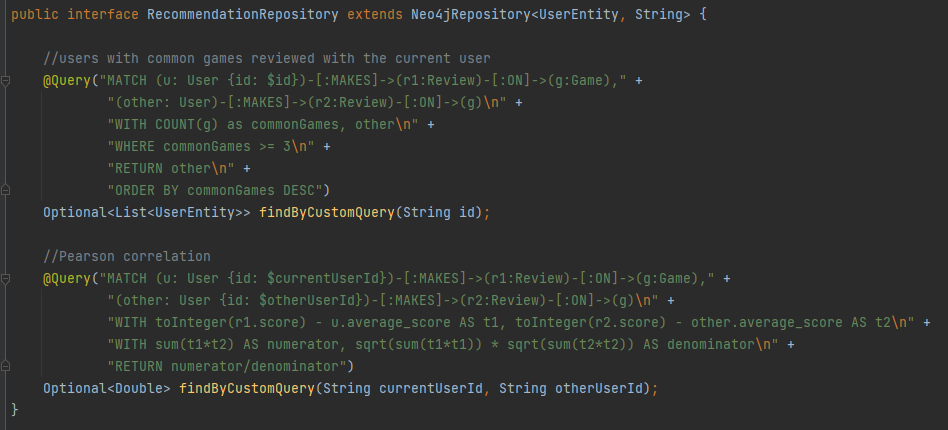
\includegraphics[scale = 0.7]{exemplu_25_recom_repository}
\caption*{}
\end{figure}

În prima interogare, vor fi furnizați acei utilizatori care au cel puțin 3 jocuri recenzate în comun cu utilizatorul căruia i se caută recomandările. Acești utilizatori sunt ordonați descrescător după criteriul menționat anterior.

A doua interogare calculează ponderea prin intermediul formulei menționate anterior. Se observă folosirea proprietății \emph{average\_score} care este actualizată prin intermediul declanșatorului explicat în capitolul 4 \textbf{Baza de date}.

\bigskip

De asemenea, o a treia interogare a fost utilizată, care furnizează acele jocuri ale utilizatorului \( i' \), împreună cu recenziile asociate, care nu sunt în comun cu jocurile recenzate de către utilizatorul \( i \). Aceste jocuri sunt cele candidat spre a fi recomandate utilizatorului \( i' \). La finalul algoritmului, aceste jocuri vor avea asociat un scor calculat prin intermediul formulei:

\[  s(i,j) = \overline{r_i} + \hat{w\_dev(i,j)}  \]

Nu am găsit o soluție pentru a executa această interogare în cadrul unei \emph{Repository}, din cauza faptului că aceasta returnează atât jocul, cât și recenzia. Așadar, am mapat manual rezultatul interogării, acest procedeu putând fi văzut în figura următoare:

\begin{figure}[H]
\centering
\caption{}
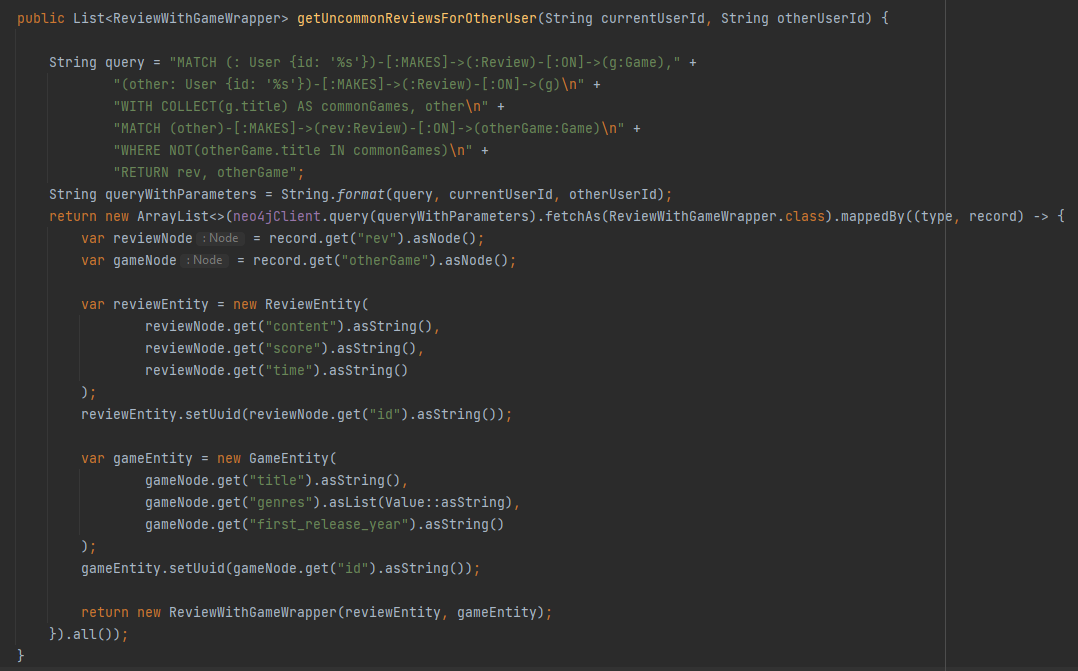
\includegraphics[scale = 0.6]{exemplu_26_third_query}
\caption*{}
\end{figure}

Așadar, aceste trei interogări au fost utilizate pentru a facilita implementarea algoritmului în limbajul Java.
Algoritmul în sine va fi ilustrat prin intermediul a trei figuri, pentru a ușura explicația și încadrarea pe pagină.

\bigskip
\textbf{Prima parte a algoritmului}
\bigskip

\begin{figure}[H]
\centering
\caption{}
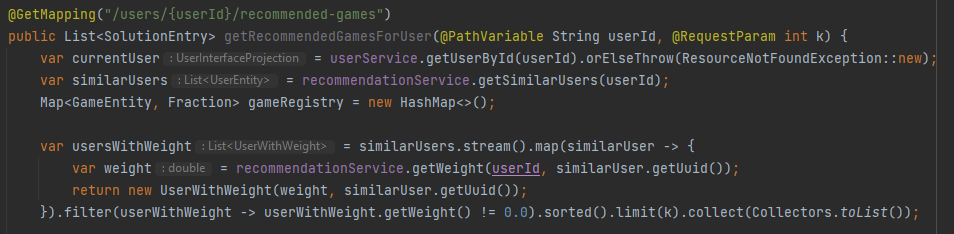
\includegraphics[scale = 0.7]{exemplu_27_first_part}
\caption*{Observație: acest algoritm a fost implementat în cadrul metodei \emph{getRecommendedGamesForUser} din \emph{GameController}}
\end{figure}

Prima parte este responsabilă de identificarea utilizatorilor similari cu utilizatorul care cere recomandarea, prin intermediul primei interogări ilustrate.

De asemenea, din acești utilizatori determinați, vor fi selectați doar acei \( k \) cu ponderile cele mai mari, acestea fiind calculate prin intermediul celei de a doua interogări prezentate. Un caz particular a fost tratat, și anume au fost ignorați acei utilizatori pentru care ponderea este egală cu \( 0 \).

În variabila \emph{gameRegistry} vor fi reținute jocurile candidat spre a fi recomandate și vor fi actualizate scorurile pe parcursul algoritmului.

\bigskip
\textbf{A doua parte a algoritmului}
\bigskip

\begin{figure}[H]
\centering
\caption{}
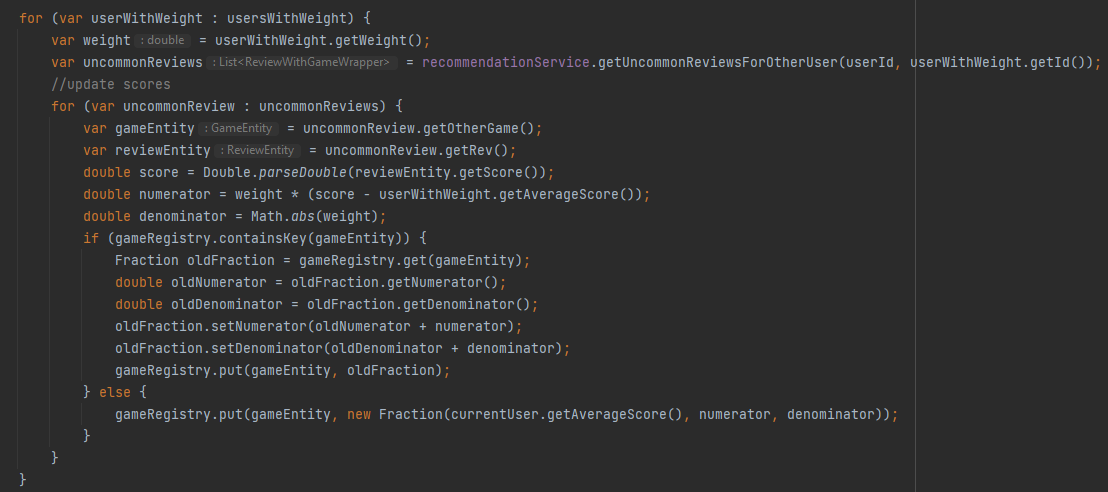
\includegraphics[scale = 0.6]{exemplu_28_second_part}
\caption*{}
\end{figure}

În această parte a algoritmului, se vor trece prin toți utilizatorii determinați la pasul anterior, iar pentru fiecare utilizator se vor determina acele jocuri recenzate care nu sunt în comun cu jocurile recenzate de utilizatorul \( i \), adică practic rezultatul celei de a treia interogări în Cypher.

Pentru fiecare joc, se calculează numărătorul și numitorul conform formulei menționate anterior, și scorul va fi actualizat corespunzător.

\newpage

\bigskip
\textbf{A treia parte a algoritmului}
\bigskip

\begin{figure}[H]
\centering
\caption{}
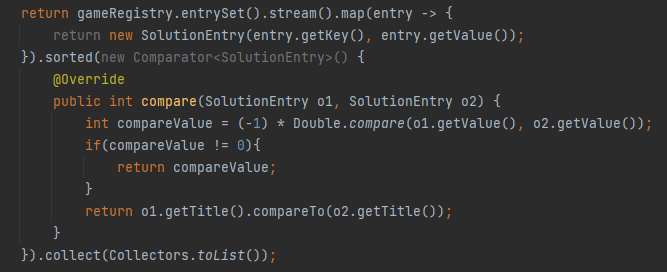
\includegraphics[scale = 0.9]{exemplu_29_third_part}
\caption*{}
\end{figure}

Această parte este responsabilă de prelucrarea soluției finale. Practic, vor fi furnizate maxim 10 jocuri ordonate descrescător după scorul obținut și crescător după titlul jocului.

\section{Front-end}

\subsection{De ce Angular?}

Angular este un \emph{framework} ce permite dezvoltarea de aplicații web la nivel de client, numite \emph{single-page}. \cite{31}.

Am ales să dezvolt partea de front-end a aplicației utilizând această tehnologie deoarece, maniera generală de lucru este realizată prin intermediul programării orientate obiect.

În această manieră, obiectele pot fi asociate cu componentele, iar o componentă în Angular este alcătuită din trei elemente principale:

\begin{enumerate}
  \item cod HTML ce reprezintă șablonul(\emph{template-ul}) componentei
  \item unul sau mai multe fișiere CSS pentru stilizarea componentei
  \item cod Typescript pentru implementarea logicii componentei(o componentă poate fi asociată intuitiv unei clase) 
\end{enumerate}

Am apreciat separarea acestor trei elemente, fiecare având un scop bine definit.

De asemenea, limbajul de programare utilizat este Typescript. Acesta este un superset al limbajului Javascript, ce adaugă suport pentru tipizare statică, aspect care permite scrierea mult mai riguroasă a codului.

\subsection{Paginile aplicației}

\bigskip
\textbf{Pagina de acasă}
\bigskip

\begin{figure}[H]
\centering
\caption{}
\begin{adjustbox}{max size={\textwidth}{\textheight}}
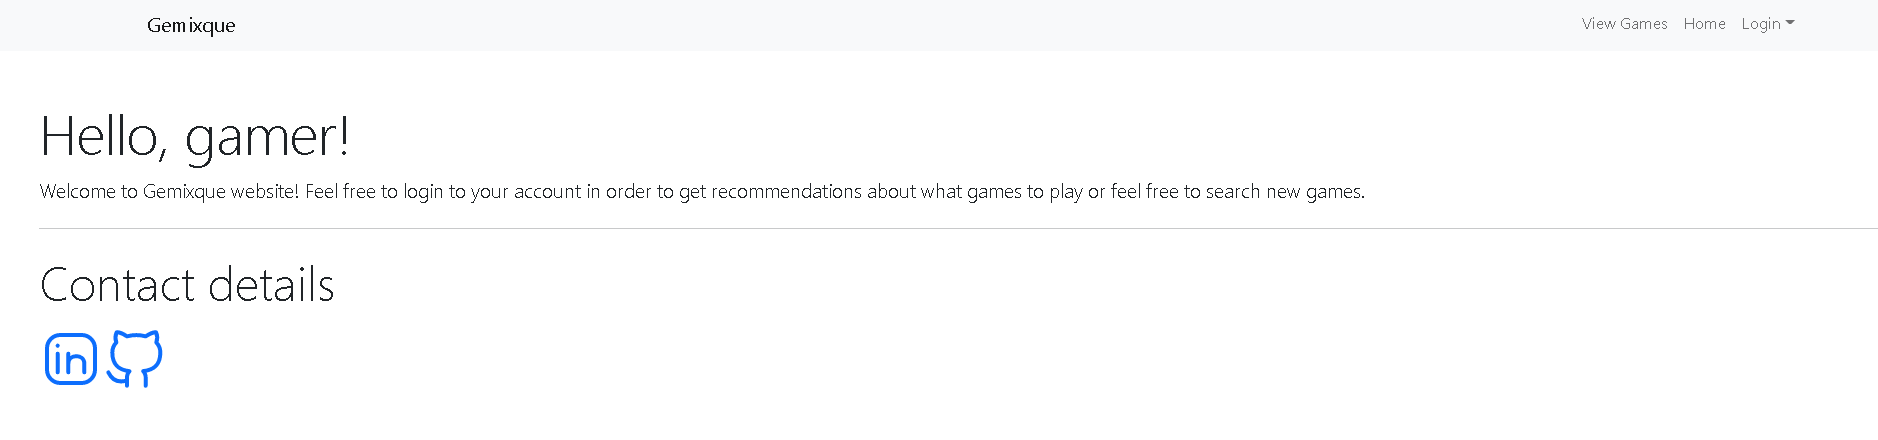
\includegraphics{exemplu_30_home_page}
\end{adjustbox}

\caption*{}
\end{figure}

În această pagină, utilizatorul este întâmpinat cu un mesaj de bun venit și cu scurte indicații legat de ce ar putea să facă în acest site. Poate ori să se logheze, pentru a-și  vedea profilul și a cere recomandări, sau poate să vizualizeze catalogul de jocuri existente.

\bigskip
\textbf{Catalogul de jocuri}
\bigskip

Această pagină poate fi accesată prin intermediul barei de navigare, mai concret prin opțiunea \emph{View Games}, și arată în felul următor:

\begin{figure}[H]
\centering
\caption{}
\begin{adjustbox}{max size={\textwidth}{\textheight}}
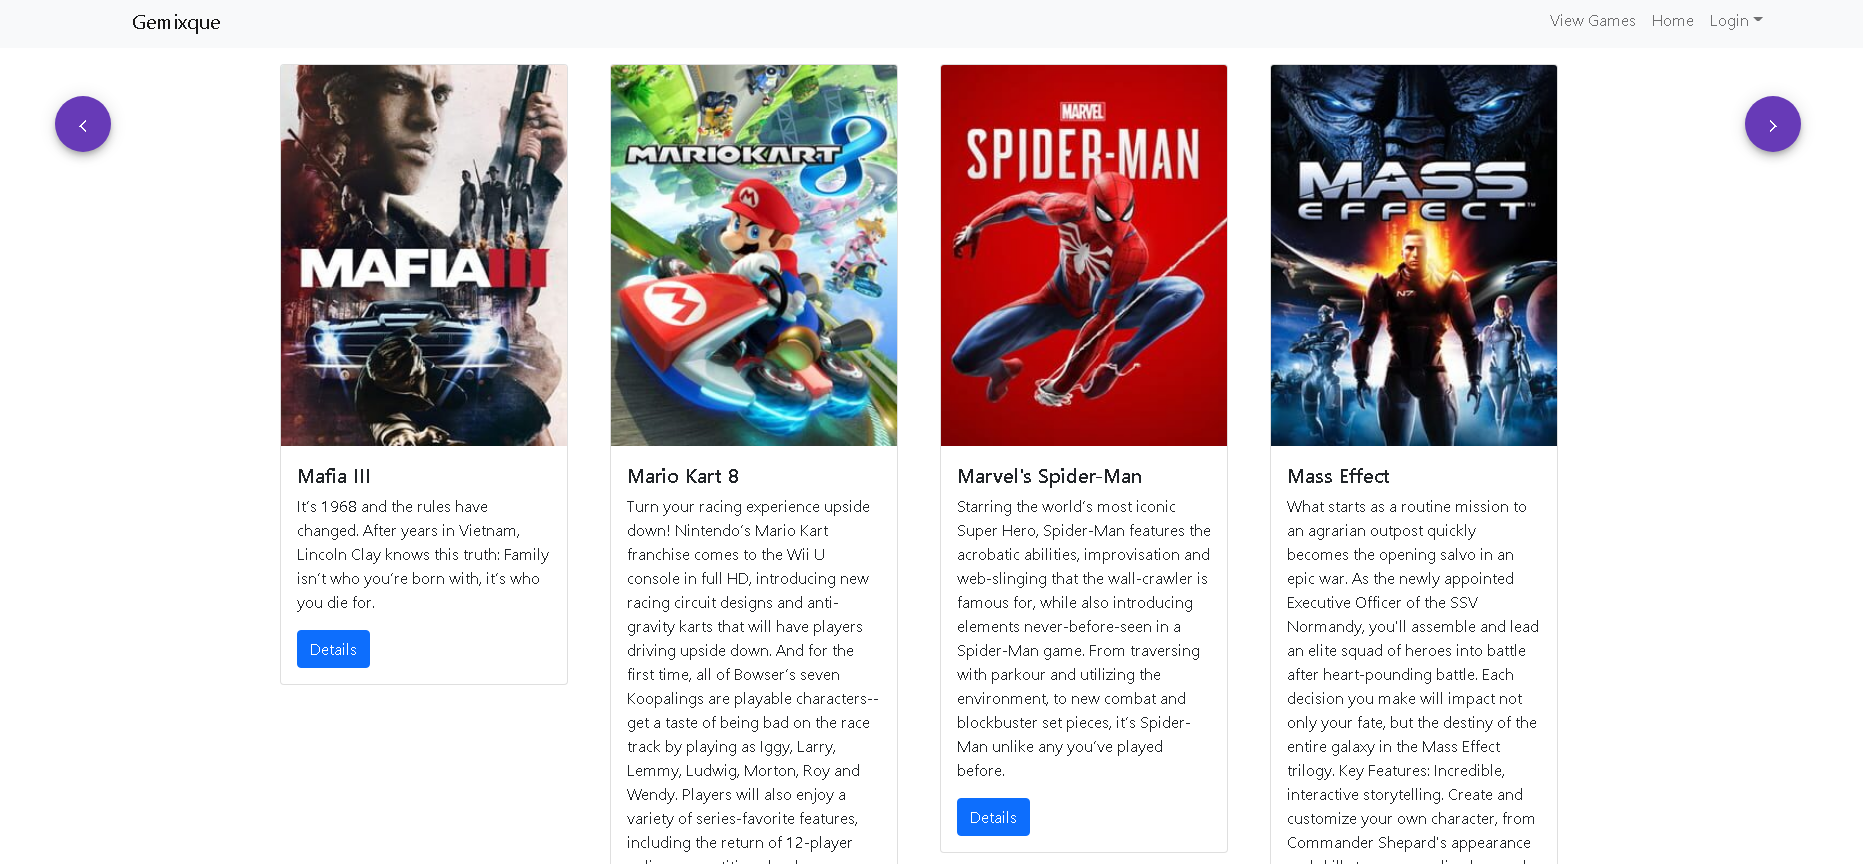
\includegraphics{exemplu_31_games_catalog}
\end{adjustbox}

\caption*{}
\end{figure}

Jocurile sunt aduse de pe \emph{back-end} prin intermediul unui \emph{request} ce suportă paginare. Acestea sunt afișate câte 8 pe  pagină(2 rânduri a câte 4 jocuri).

Înainte de a fi prezentată următoarea pagină, vor fi descrise anumite concepte din \emph{framework-ul} Angular care au facilitat atât crearea acestei pagini, cât și a celor care vor urma a fi ilustrate.

\bigskip
\textbf{Servicii, observabile și tratarea acestora}
\bigskip

În primul rând, pentru a utiliza \emph{request-urile} ce au fost implementate pe \emph{back-end}, am implementat servicii pe partea de \emph{front-end}. Un serviciu este o clasă separată de componentă, și are în general rolul de a efectua anumite funcționalități specifice. \cite{32}

De exemplu, pentru pagina anterior menționată, am implementat un serviciu care se ocupă de obținerea jocurilor prin paginare. Acesta arată în felul următor:

\begin{figure}[H]
\centering
\caption{}
\begin{adjustbox}{max size={\textwidth}{\textheight}}
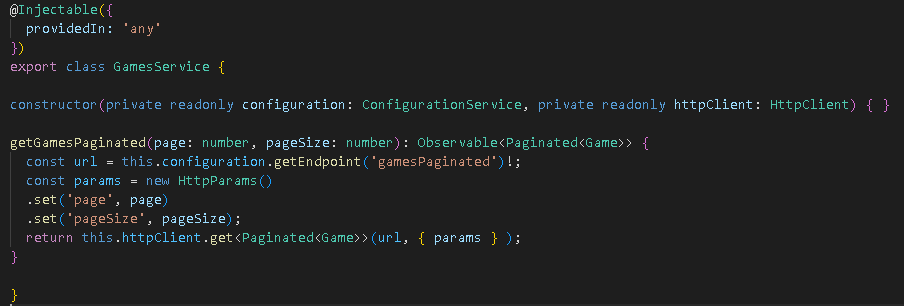
\includegraphics{exemplu_32_games_paginated_service}
\end{adjustbox}

\caption*{}
\end{figure}

În primul rând se observă folosirea adnotării \emph{Injectable}, care indică faptul că instanța clasei poate fi injectată. Acest serviciu va fi instanțiat automat atunci când este folosit ca parametru în cadrul unui constructor.

De asemenea, se observă alte două servicii injectate în constructorul acestui serviciu, anume \emph{ConfigurationService} și \emph{HttpClient}. Primul este implementat de mine, și are ca scop extragerea \emph{url-ului} corespunzător dintr-un fișier în format JSON în care am reținut toate \emph{url-urile} asociate \emph{request-urilor} de pe \emph{back-end}.

Al doilea serviciu este oferit de Angular, și este responsabil de efectuarea \emph{request-urilor} prin intermediul protocolului Http.

În metoda \emph{getGamesPaginated}, se extrage url-ul corespunzător \emph{request-ului} care va furniza jocurile prin paginare, se setează \emph{query parameters} corespunzători și se va returna un observabil.

Acest observabil face o trimitere la \emph{design pattern-ul} numit \emph{observer}, în care un obiect(subiect) emite anumite evenimente, iar unul sau mai mulți ascultători(observatori) vor fi notificați de către subiect. \cite{33}

Scopul folosirii acestui \emph{design pattern} în Angular este de a rezolva problema tratării evenimentelor asincrone. De menționat faptul că returnarea observabilului de către serviciu nu implică și efectuarea \emph{request-lui} corespunzător. Acest observabil este consumat doar atunci când se va apela metoda \emph{subscribe}.

Serviciul anterior menționat va fi consumat în cadrul paginii ce afișează catalogul de jocuri. Mai concret, în cadrul clasei \emph{GamesComponent}, în felul următor:

\begin{figure}[H]
\centering
\caption{}
\begin{adjustbox}{max size={\textwidth}{\textheight}}
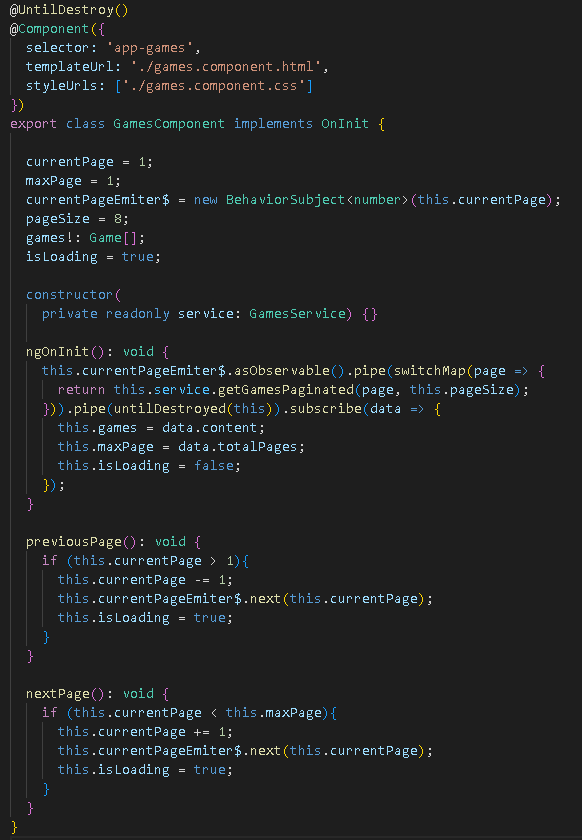
\includegraphics{exemplu_33_subscribe}
\end{adjustbox}

\caption*{}
\end{figure}

În cadrul acestei componente, se observă implementarea interfeței funcționale \emph{OnInit} prin implementarea metodei \emph{ngOnInit}. 

În general, o componentă are o serie de evenimente prin care cu ajutorul implementării unor anumite interfețe funcționale, se pot efectua acțiuni atunci când se declanșează aceste evenimente.  \cite{34}

În exemplul din figură, se dorește obținerea jocurilor prin paginare atunci când se inițializează componenta. În primul rând, pentru a trata în mod asincron schimbarea paginii curente, se folosește un \emph{BehaviorSubject}, prin care se pot emite evenimente prin apelarea metodei \emph{next}.

În general, înainte ca un observabil să fie consumat, se pot folosi operatori care vor prelucra datele emise de acel observabil înainte să ajungă să fie consumate. Acești operatori sunt înlănțuiți în cadrul metodei \emph{pipe}. Librăria RxJS \cite{35} vine la pachet cu Angular și oferă o gamă variată de operatori.

În cadrul metodei \emph{ngOnInit}, acel \emph{BehaviorSubject} menționat anterior este convertit într-un observabil. Pentru a putea obține jocurile atunci când s-a schimbat pagina, se poate folosi operatorul \emph{switchMap}, care schimbă observabilul anterior în acel observabil care este responsabil de obținerea de jocuri. De asemenea, operatorul \emph{untilDestroyed} este folosit pentru a asigura faptul că atunci când se va ieși de pe pagina cu catalogul de jocuri(adică atunci când se distruge instanța clasei \emph{GamesComponent}), nu se vor mai asculta alte evenimente, deci observabilul va fi completat.

În cadrul metodei \emph{subscribe}, se vor prelua datele și vor fi reținute pentru a putea fi afișate eventual în șablonul componentei.

\bigskip
\textbf{Pagina unui joc}
\bigskip

Atunci când utilizatorul vizualizează catalogul și dorește să vadă în detaliu informații despre un anumit joc, va fi întâmpinat cu următoarea pagină:

\begin{figure}[H]
\centering
\caption{}
\begin{adjustbox}{max size={\textwidth}{\textheight}}
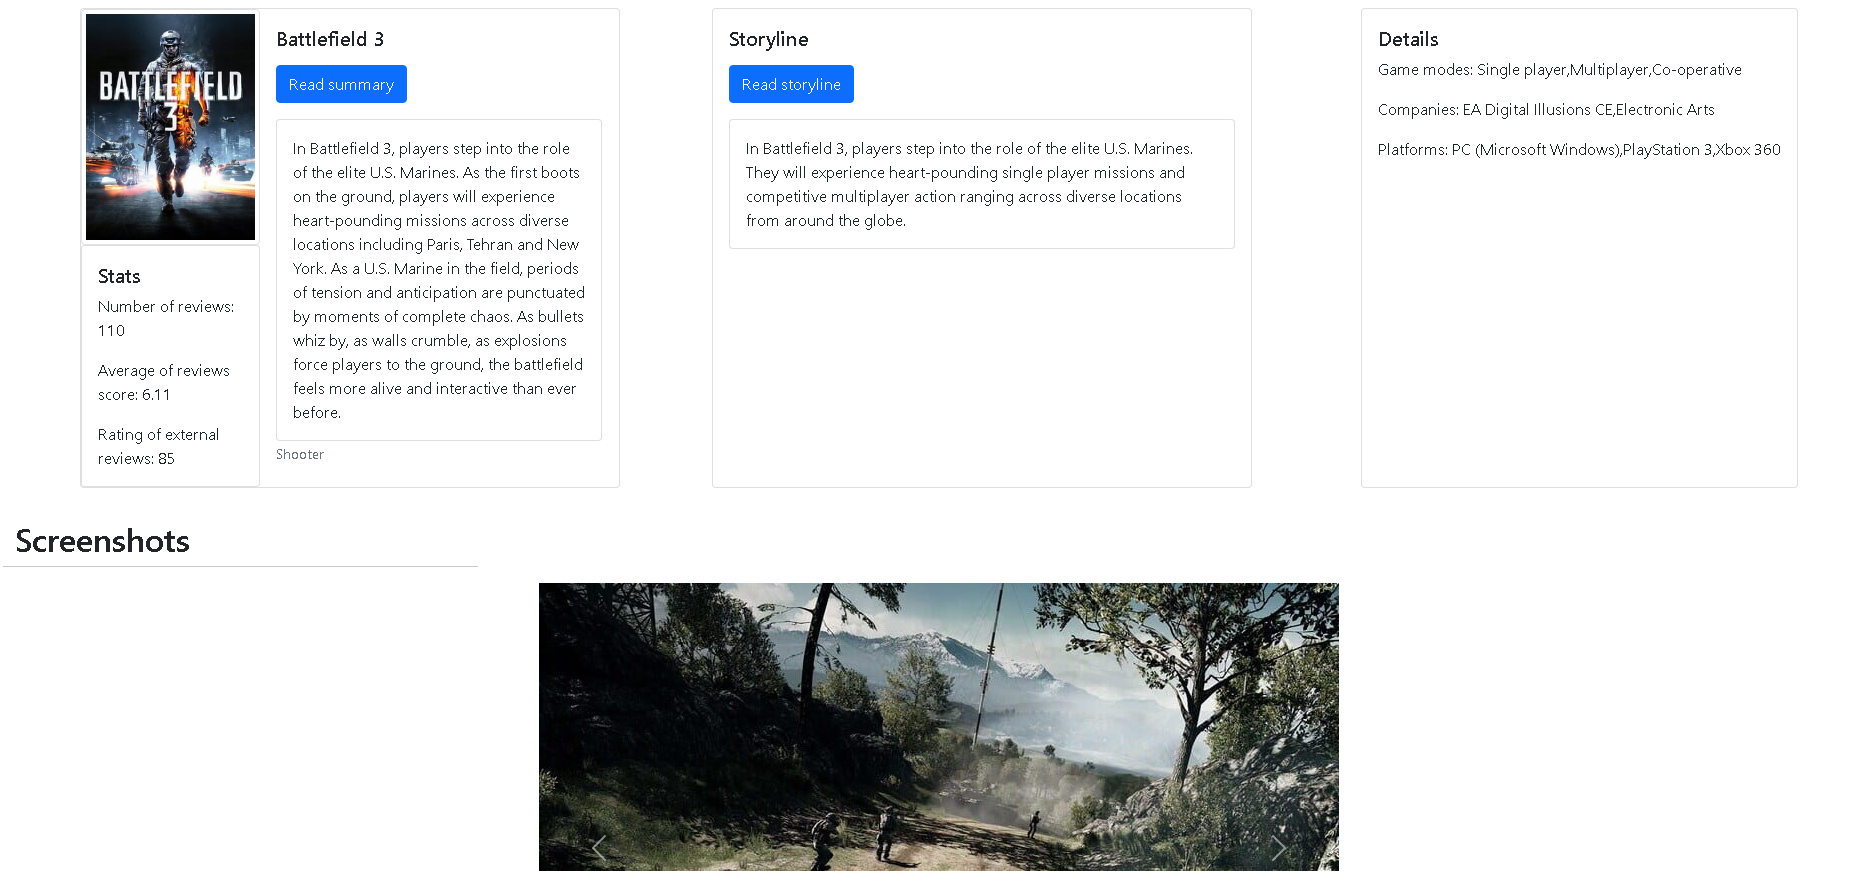
\includegraphics{exemplu_34_game_details}
\end{adjustbox}

\caption*{}
\end{figure}

\begin{figure}[H]
\centering
\caption{}
\begin{adjustbox}{max size={\textwidth}{\textheight}}
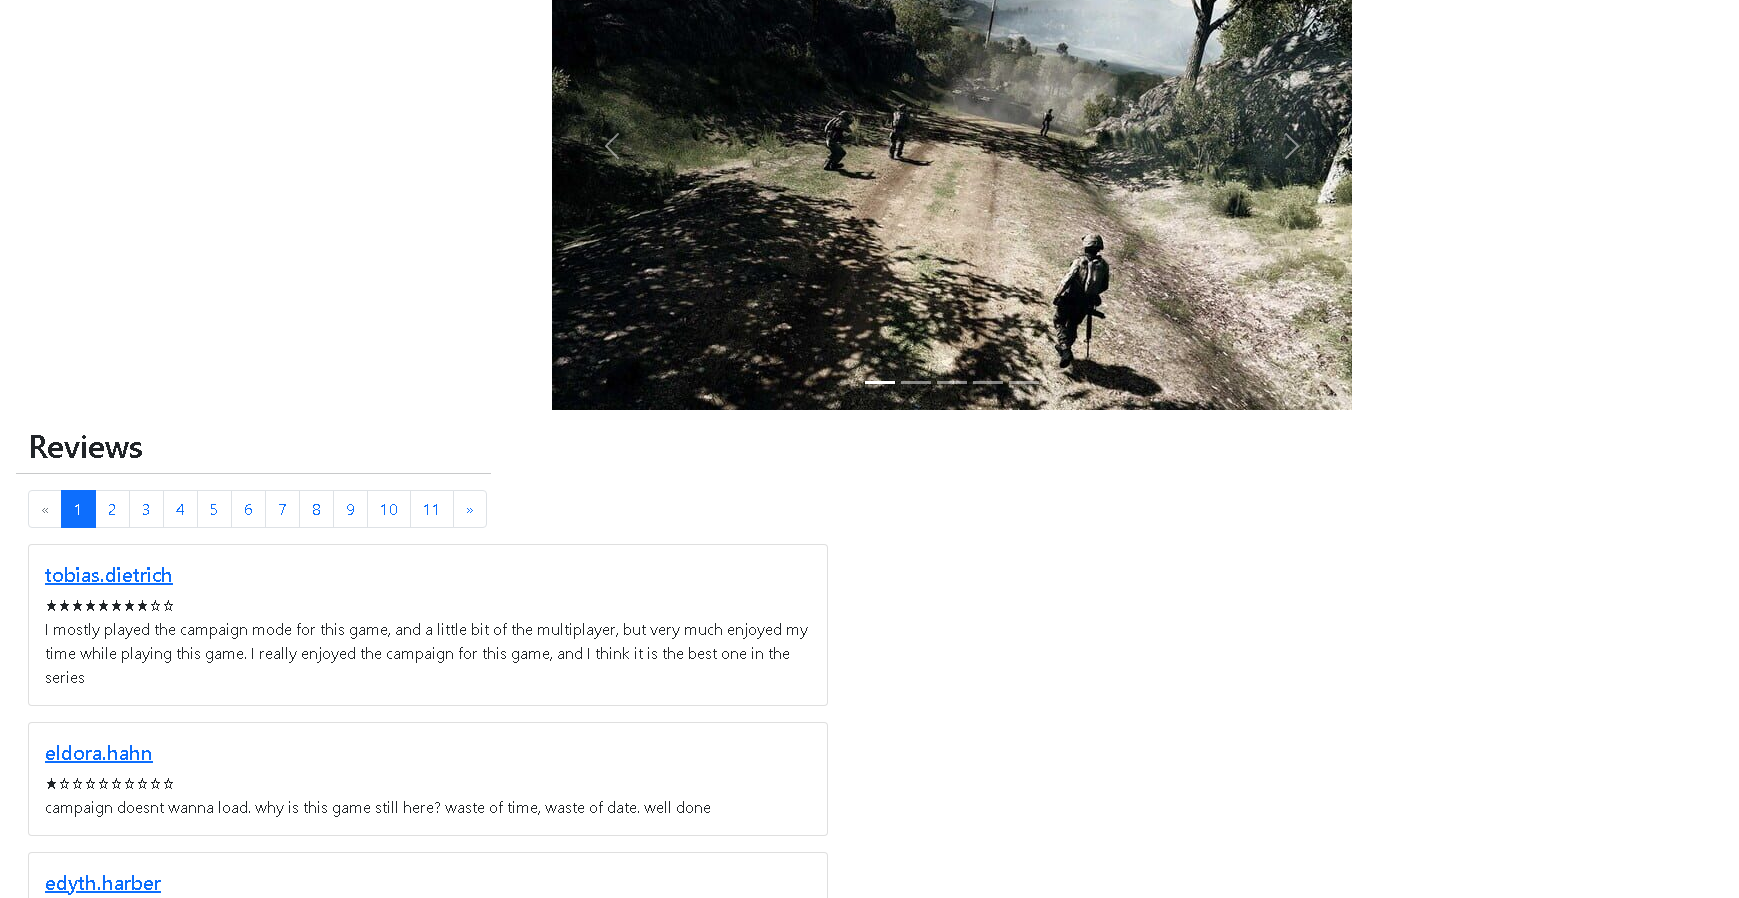
\includegraphics{exemplu_35_game_details_2}
\end{adjustbox}

\caption*{}
\end{figure}

\bigskip
\textbf{Profilul unui utilizator}
\bigskip

În stadiul actual, un utilizator care nu este logat poate să privească profilul altui utilizator(de exemplu, cel care a făcut o anumită recenzie), însă ca să poată să primească recomandări, trebuie să se logheze în aplicație.

În cazul în care credențialele introduse de utilizator sunt incorecte, atunci o notificare va fi afișată care să sugereze acest lucru. În caz contrar, \emph{request-ul} de pe \emph{back-end} va furniza un \emph{token} care va fi reținut în \emph{local storage-ul} \emph{browser-ului} pentru a persista starea de logare.
 
 După o logare efectuată cu succes, profilul arată după cum urmează:

\begin{figure}[H]
\centering
\caption{}
\begin{adjustbox}{max size={\textwidth}{\textheight}}
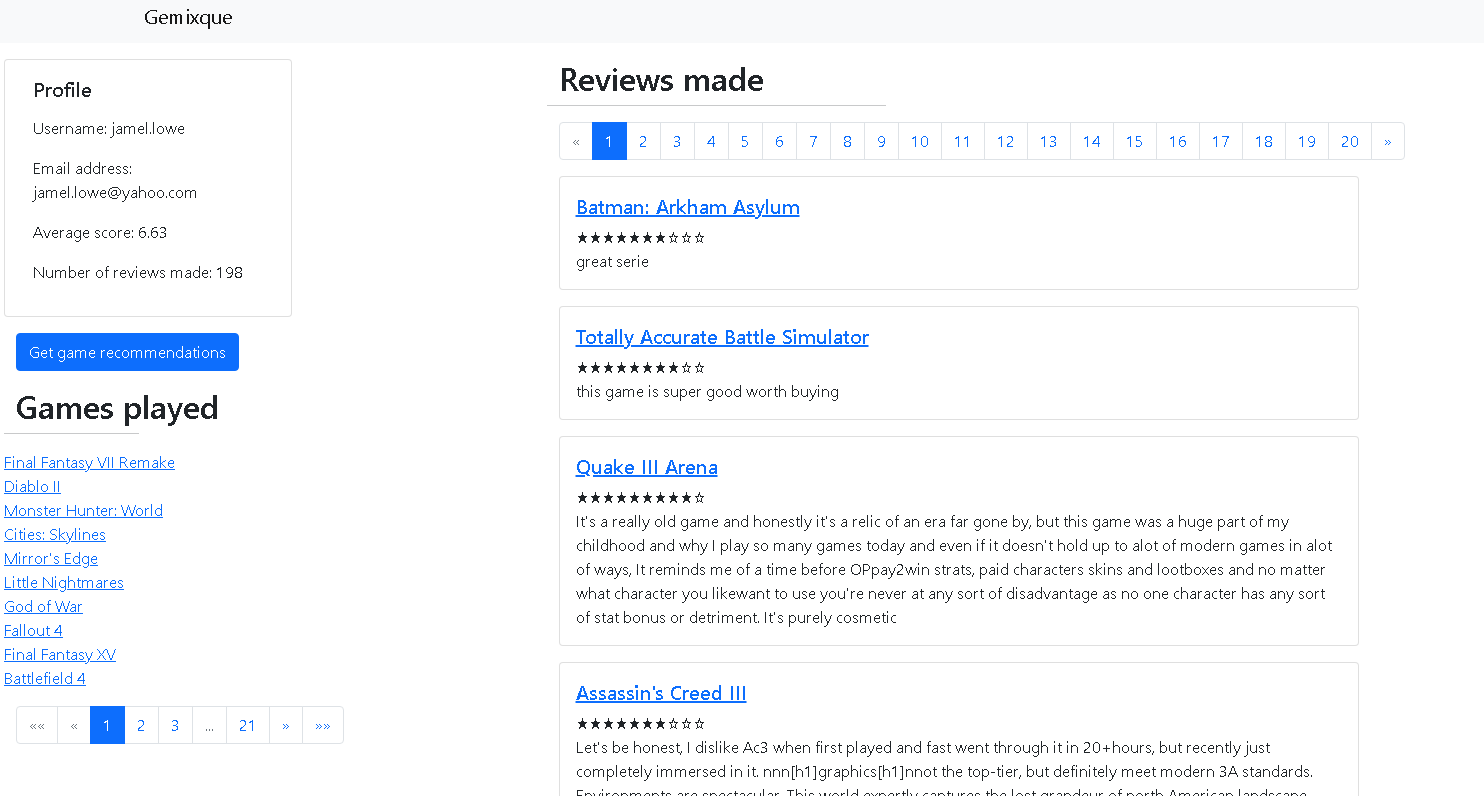
\includegraphics{exemplu_36_profile}
\end{adjustbox}

\caption*{}
\end{figure}

\bigskip
\textbf{Afișarea rezultatelor algoritmului de recomandare}
\bigskip

Prin apăsarea butonului \emph{Get game recommendations}, o nouă fereastră va fi deschisă prin care utilizatorul va putea seta parametrul \( k \) pentru a controla precizia algoritmului. Inițial, înainte de afișarea rezultatelor, fereastra arată în felul următor:

\begin{figure}[H]
\centering
\caption{}
\begin{adjustbox}{max size={\textwidth}{\textheight}}
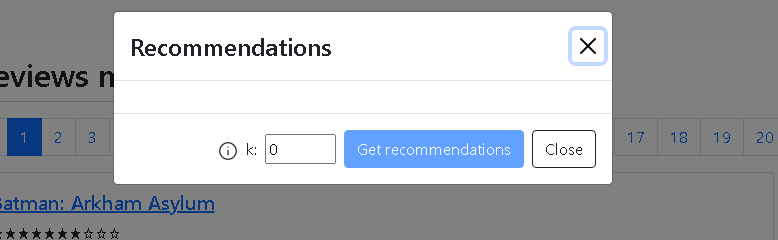
\includegraphics{exemplu_37_modal_1}
\end{adjustbox}

\caption*{Acel \emph{icon} plasat în fața lui k are rol informativ. Atunci când utilizatorul va acoperi acel \emph{icon} cu \emph{mouse-ul}, un text va apărea, prin care este precizat intervalul prin care poate fi setat k(adică între 1 și 50). De reamintit faptul că acest parametru indică numărul de utilizatori care vor fi luați în considerare în generarea rezultatelor. Cu alte cuvinte, cu cât k este mai mare, cu atât mai multe jocuri vor fi luate în considerare.}
\end{figure}

După aceea, prin apăsarea butonului \emph{Get recommendations}, se vor încărca datele și inițial vor apărea rezultatele sub forma unui tabel:

\begin{figure}[H]
\centering
\caption{}
\begin{adjustbox}{max size={\textwidth}{\textheight}}
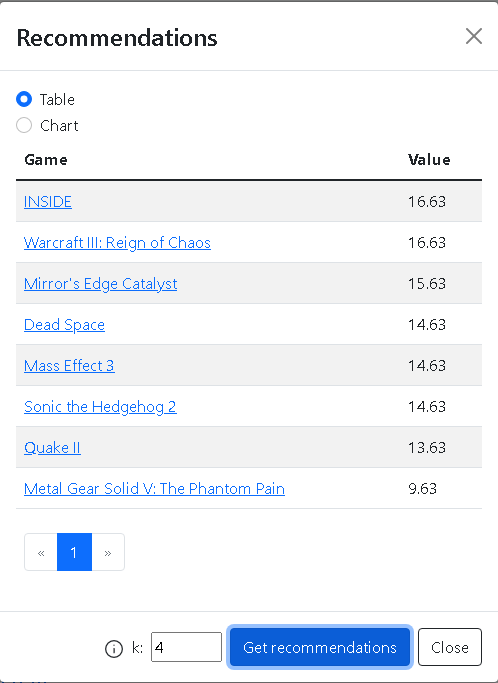
\includegraphics[scale=0.55]{exemplu_38_modal_2}
\end{adjustbox}

\end{figure}

\emph{Request-ul} de pe back-end oferă deja sortate descrescător jocurile după valoarea calculată. Acest tabel arată jocurile obținute pentru un anumit parametru k.

Însă, dacă se dorește schimbarea opțiunii de vizualizare a rezultatelor, se poate selecta opțiunea \emph{Chart}.

Inițial, după o primă generare, graficul arată în felul următor:

\begin{figure}[H]
\centering
\caption{}
\begin{adjustbox}{max size={\textwidth}{\textheight}}
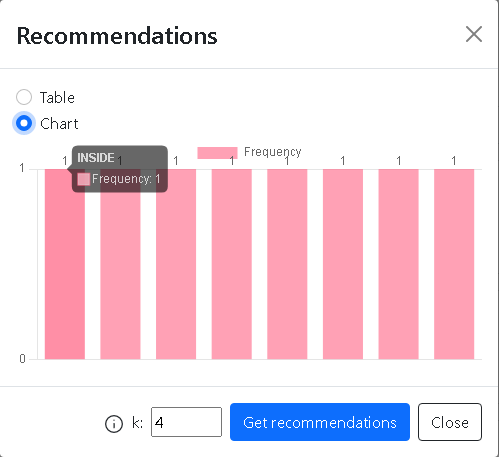
\includegraphics[scale=0.7]{exemplu_39_modal_3}
\end{adjustbox}
\caption*{Pentru a genera acest grafic, am folosit librăria \emph{ng2-charts} \cite{36} }
\end{figure}

Acest grafic are scopul de a arăta care jocuri apar de cele mai multe ori în tabel cu cât se generează mai multe rezultate prin schimbarea parametrului k. Dacă se încearcă generarea cu același parametru k, atunci nu are rost ca acest grafic să fie actualizat, căci rezultatele sunt aceleași. (în teorie, rezultatele ar putea să fie schimbate pentru același k dacă unul din cei k utilizatori va modifica nota unei recenzii, sau va adăuga o nouă recenzie înainte ca utilizatorul să declanșeze execuția algoritmului)

După câteva generări, graficul ar putea arăta astfel:

\begin{figure}[H]
\centering
\caption{}
\begin{adjustbox}{max size={\textwidth}{\textheight}}
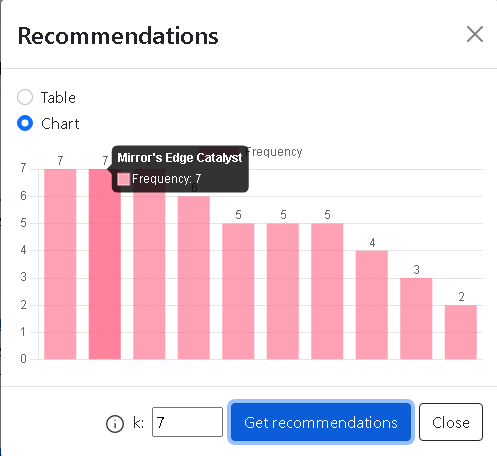
\includegraphics[scale=1]{exemplu_40_modal_4}
\end{adjustbox}
\caption*{}
\end{figure}

Rezultatele din grafic au fost generate în această manieră ca utilizatorul să poată tragă concluzii mult mai ușor legat de ce jocuri să aleagă. Cu alte cuvinte, utilizatorul poate mult mai ușor să analizeze rezultatele după mai multe schimbări ale parametrului k.


\section{Manual de utilizare}

Toate fișierele ce sunt necesare pentru instalarea locală a aplicației se găsesc în arhiva \emph{surse.zip}.

\newpage

\bigskip
\textbf{Instalarea și pornirea bazei de date}
\bigskip

\begin{enumerate}
  \item Instalarea aplicației desktop Neo4j
  
  Se va accesa următorul \emph{link} pentru a se descărca aplicația desktop: 
  
  \url{https://neo4j.com/download-center/#desktop}
  
  Înainte de a se începe descărcarea, trebuie introduse următoarele credențiale cu scopul primirii unei chei ce va fi introdusă pentru a activa o licență valabilă timp de un an.
  
  \begin{figure}[H]
\centering
\caption{}
\begin{adjustbox}{max size={\textwidth}{\textheight}}
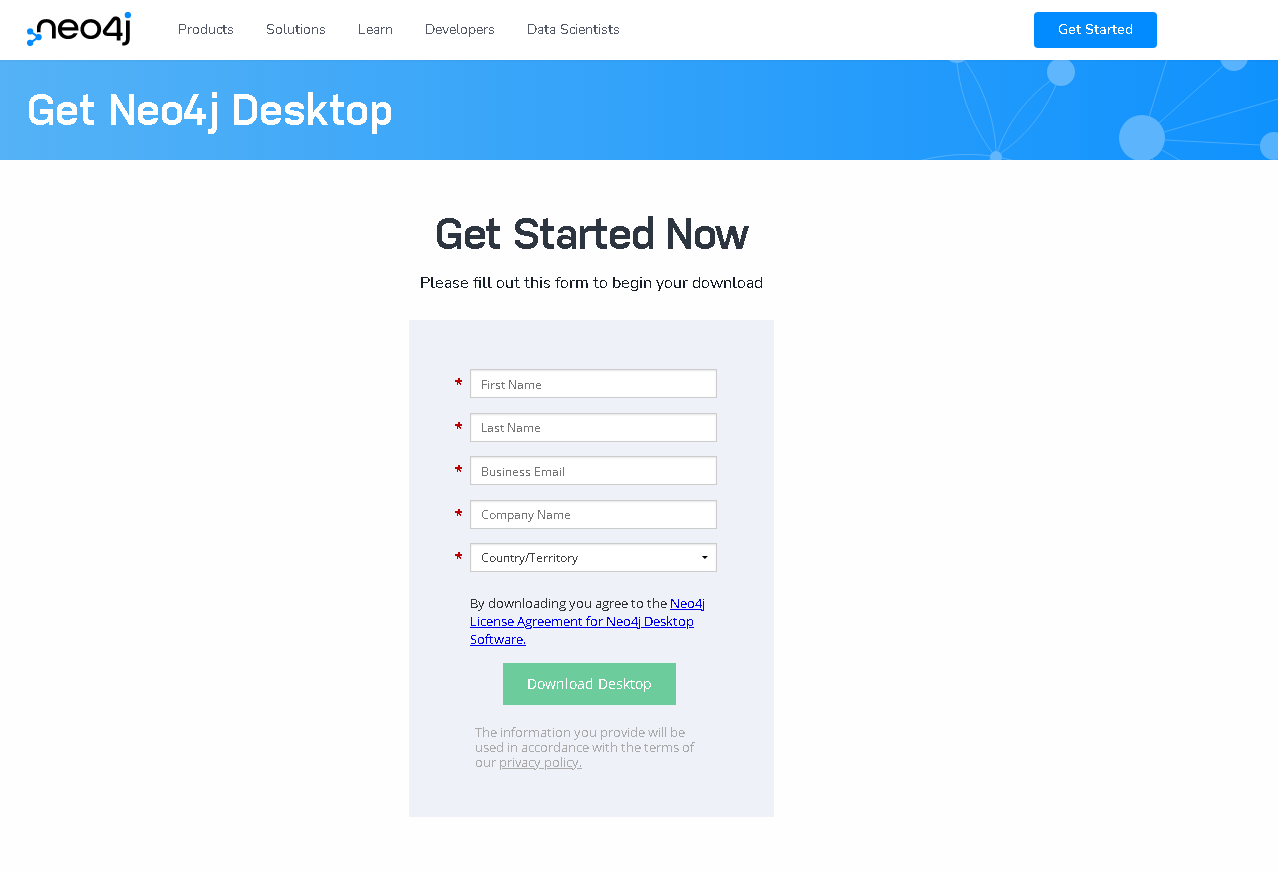
\includegraphics[scale=1]{exemplu_41_neo4j_credentiale}
\end{adjustbox}
\caption*{}
\end{figure}

   
  Se pot urmări pașii de instalare din acest videoclip pentru sistemul de operare Windows:
  
  \url{https://www.youtube.com/watch?v=RSbhmVF_ccs}
  
  
  \item Importarea bazei de date
  
  Fișierele necesare ce vor fi importate se regăsesc în directorul \emph{dumps}. Aceste fișiere sunt următoarele: neo4j.dump și system.dump.
  
  Înainte de a fi importate aceste fișiere, se va crea un nou proiect, apăsând butonul \emph{New} și secțiunea \emph{Create project}:
  
\begin{figure}[H]
\centering
\caption{}
\begin{adjustbox}{max size={\textwidth}{\textheight}}
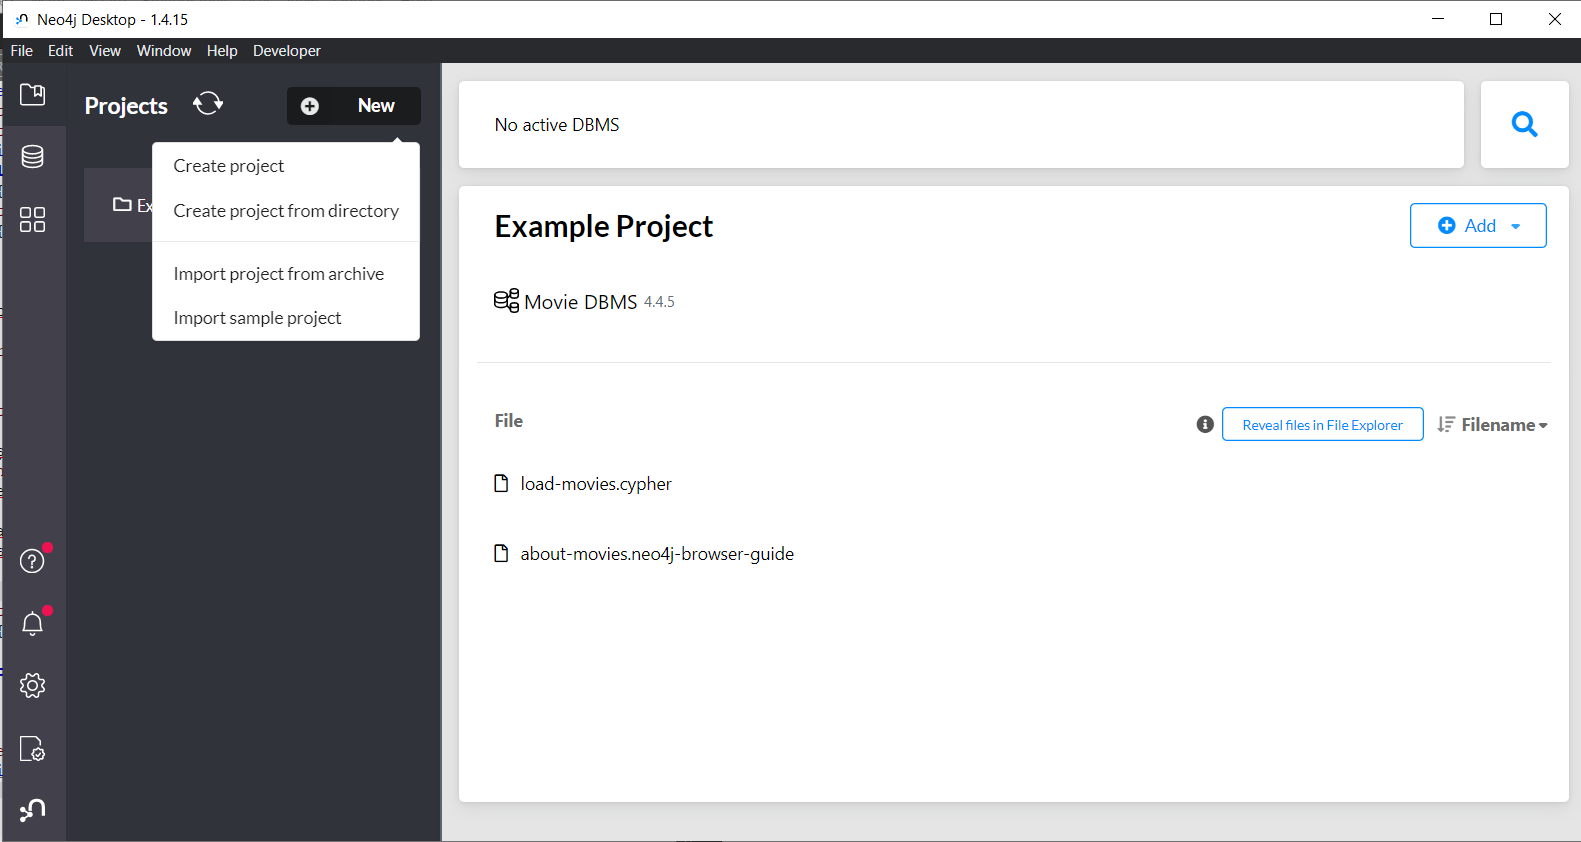
\includegraphics[scale=1]{exemplu_42_new_project}
\end{adjustbox}
\caption*{}
\end{figure}

  După ce s-a creat acest proiect, pentru început numele acestuia poate fi schimbat. Pentru conveniență, se poate redenumi proiectul în \emph{Gemixque}.
  
  În cadrul acestui proiect, se va adăuga o nouă bază de date prin apăsarea butonului \emph{Add} și a secțiunii \emph{Local DBMS}.
  
\begin{figure}[H]
\centering
\caption{}
\begin{adjustbox}{max size={\textwidth}{\textheight}}
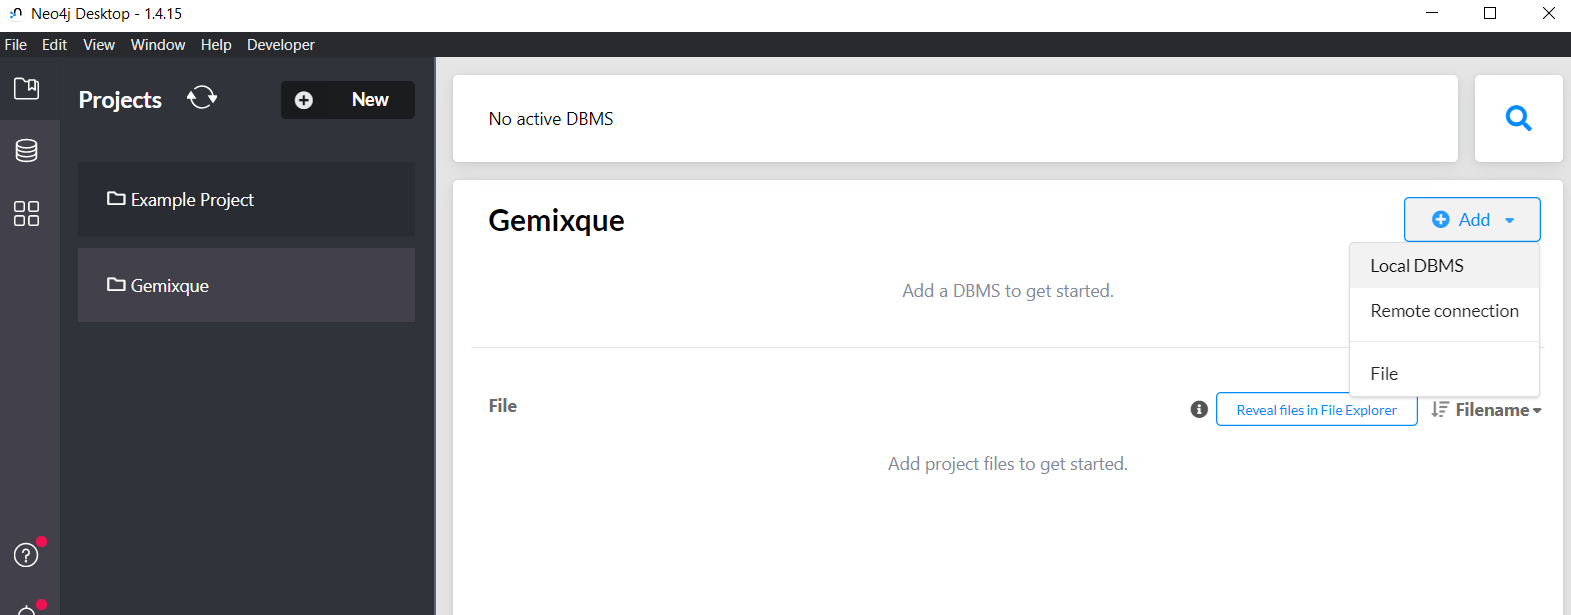
\includegraphics[scale=1]{exemplu_43_new_database}
\end{adjustbox}
\caption*{}
\end{figure}

\newpage
  După acest pas, se vor introduce următoarele informații:
  
  \begin{figure}[H]
\centering
\caption{}
\begin{adjustbox}{max size={\textwidth}{\textheight}}
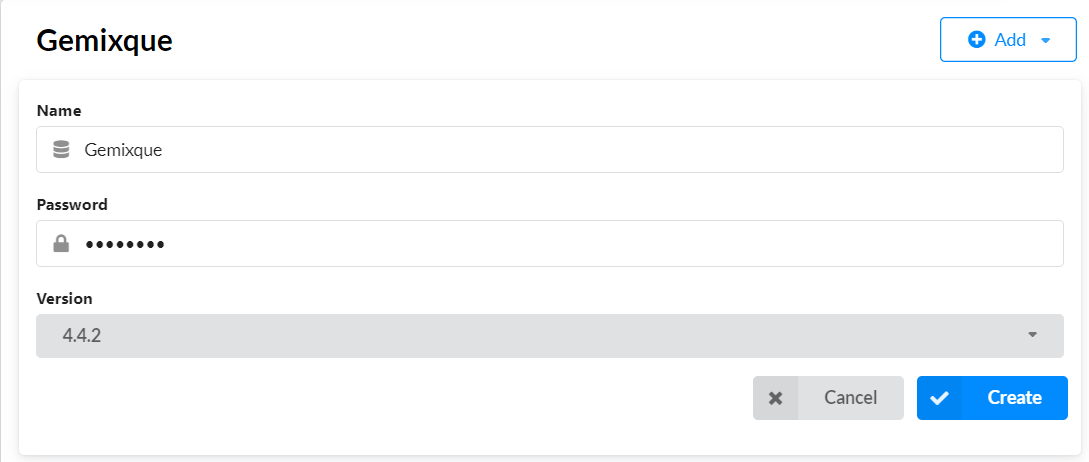
\includegraphics[scale=1]{exemplu_44_add_database}
\end{adjustbox}
\caption*{Numele: \emph{Gemixque}, parola dorită și versiunea 4.4.2}
\end{figure}

  Se apasă pe butonul \emph{Create} și se va aștepta până când baza de date va fi creată.
  
  Urmează importarea acelor fișiere \emph{dump} anterior menționate. Pentru a realiza acest lucru, se va deschide un terminal în felul următor:
  
    \begin{figure}[H]
\centering
\caption{}
\begin{adjustbox}{max size={\textwidth}{\textheight}}
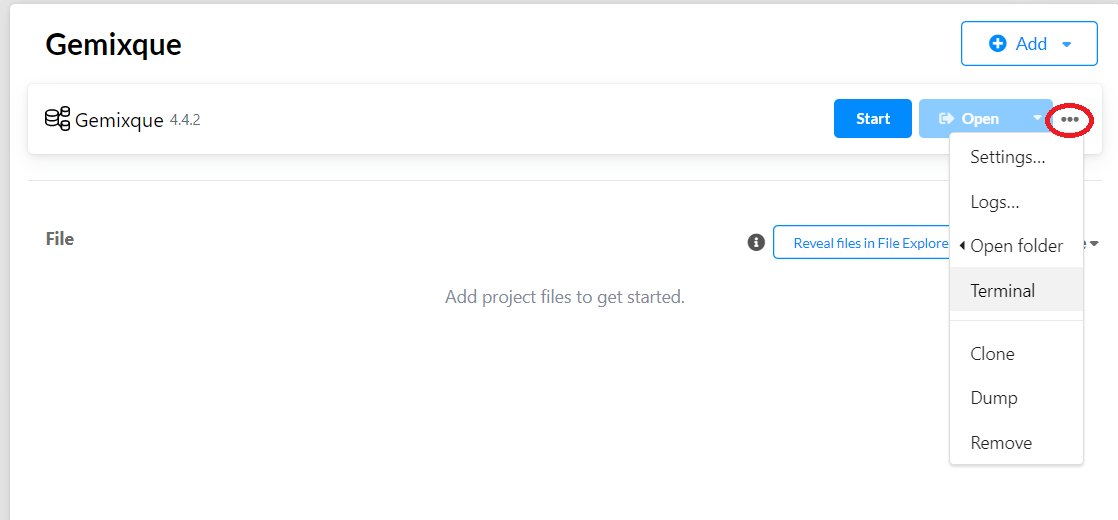
\includegraphics[scale=1]{exemplu_45_terminal}
\end{adjustbox}
\caption*{}
\end{figure}
  
  După deschiderea terminalului, se va executa următoarea comandă pentru importarea acelor fișiere:
  
      \begin{figure}[H]
\centering
\caption{}
\begin{adjustbox}{max size={\textwidth}{\textheight}}
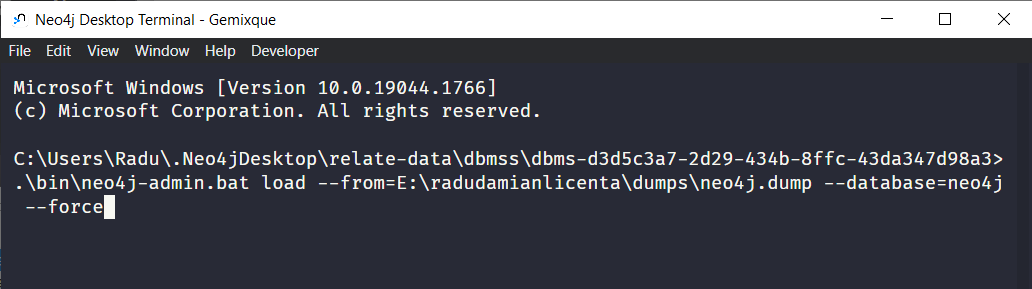
\includegraphics[scale=1]{exemplu_46_load_command}
\end{adjustbox}
\caption*{În opțiunea \emph{from} se va introduce calea către fișierul \emph{dump} corespunzător. În mod analog se va executa comanda și pentru fișierul system.dump}
\end{figure}
  
  
  
  \item Verificarea importării bazei de date
  
  Pentru a verifica dacă baza de date s-a importat corect, în primul rând se va apăsa pe butonul de \emph{Start} pentru a porni baza de date.
  
  După acest pas, se va deschide panoul de comandă pentru a verifica dacă datele sunt existente conform schemei bazei de date. Se va apăsa butonul \emph{Open} $\rightarrow$ \emph{Neo4j Browser} :
  
        \begin{figure}[H]
\centering
\caption{}
\begin{adjustbox}{max size={\textwidth}{\textheight}}
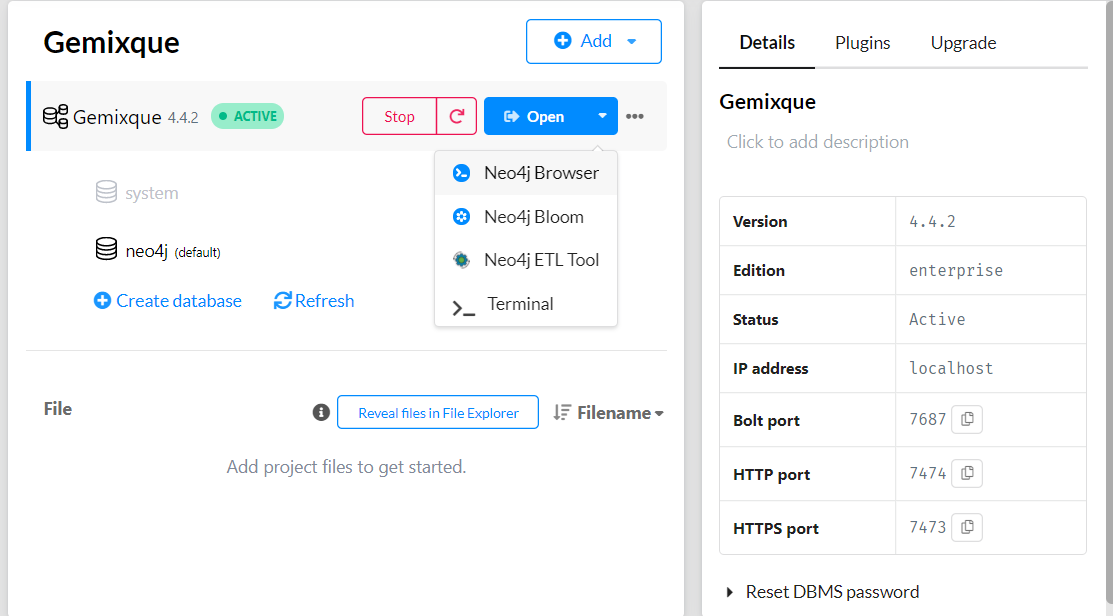
\includegraphics[scale=1]{exemplu_47_open}
\end{adjustbox}
\caption*{}
\end{figure}

\newpage
În panoul de comandă, ar trebui să se regăsească următoarele date:

        \begin{figure}[H]
\centering
\caption{}
\begin{adjustbox}{max size={\textwidth}{\textheight}}
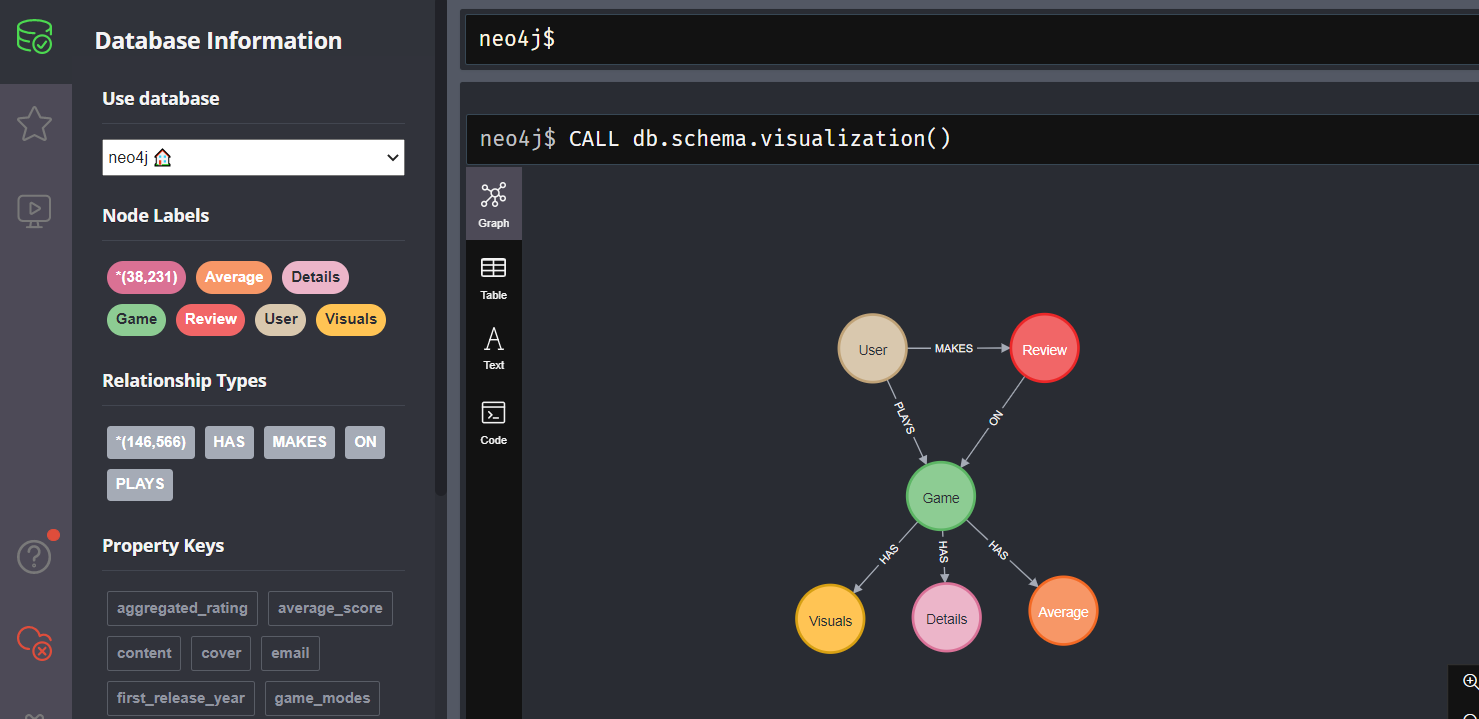
\includegraphics[scale=1]{exemplu_48_verificare}
\end{adjustbox}
\caption*{}
\end{figure}
  
  
\end{enumerate}

\bigskip
\textbf{Pornirea serverului de back-end}
\bigskip

Fișierele corespunzătoare serverului de \emph{back-end} se regăsesc în directorul \emph{gemixque-api}

Pentru a facilita pornirea serverului, am folosit un IDE pentru a deschide proiectul. Am folosit IDE-ul Intellij IDEA varianta Community, însă oricare IDE poate fi ales care să suporte aplicații implementate în Java.

Pentru a porni acest server local, se va apăsa click-dreapta pe fișierul \emph{GemixqueApiApplication} și se va apăsa secțiunea următoare:

        \begin{figure}[H]
\centering
\caption{}
\begin{adjustbox}{max size={\textwidth}{\textheight}}
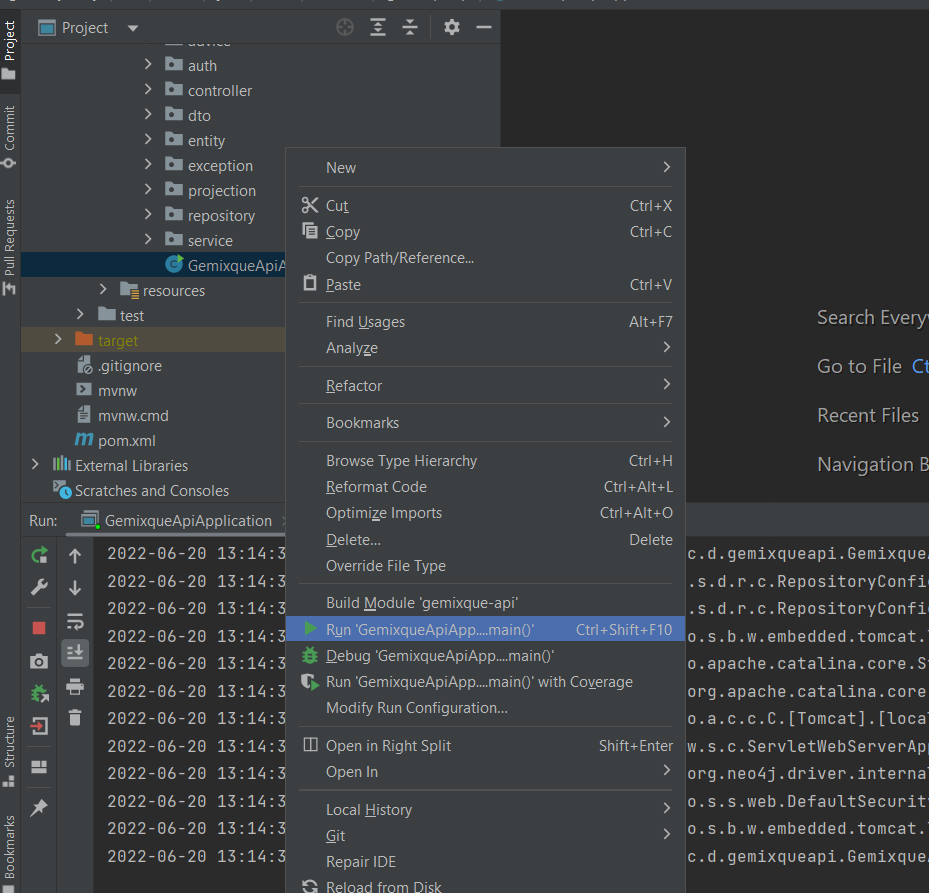
\includegraphics[scale=0.6]{exemplu_49_open_backend}
\end{adjustbox}
\caption*{Prima executare s-ar putea să dureze un timp relativ semnificativ, deoarece se descarcă dependențele necesare proiectului.}
\end{figure}

\bigskip
\textbf{Pornirea serverului de front-end}
\bigskip

Fișierele corespunzătoare serverului de \emph{front-end} se regăsesc în directorul \emph{gemixque-ui}.

Pentru început, trebuie descărcat \emph{NodeJs}, care vine la pachet cu utilitarul npm utilizat pentru gestionarea dependențelor unui proiect implementat în Javascript.

\url{https://nodejs.org/en/download/}

După aceea, se deschide un terminal în interiorul directorului \emph{gemixque-ui}. Se va executa următoarea comandă pentru a instala inițial dependențele necesare:

        \begin{figure}[H]
\centering
\caption{}
\begin{adjustbox}{max size={\textwidth}{\textheight}}
\includegraphics[scale=0.8]{exemplu_50_npm}
\end{adjustbox}
\caption*{}
\end{figure}

După ce s-au instalat dependențele, se poate executa comanda \emph{npm start} pentru a porni serverul de \emph{front-end}. Dacă totul s-a efectuat cu succes, atunci ar trebui să se deschidă automat un nou \emph{tab} în \emph{browser-ul} implicit cu pagina de acasă a aplicației.


\section{Concluzii și direcții viitoare}



\renewcommand\bibname{Bibliografie}
\begin{thebibliography}{9}

\bibitem{igdb-api}
  
  \textit{IGDB API}
  
  \url{https://www.igdb.com/api}
  
  \url{https://github.com/husnjak/IGDB-API-JVM}
  
\bibitem{steam-reviews}
  
  \textit{Steamworks Documentation - Reviews}
  
  \url{https://partner.steamgames.com/doc/store/getreviews}
  
\bibitem{java-faker}
  
  \textit{Java Faker}
  
  \url{https://github.com/DiUS/java-faker}
  
\bibitem{apache-commons-csv}
  
  \textit{Apache Commons CSV}
  
  \url{https://commons.apache.org/proper/commons-csv/}


\bibitem{lamport94}
  
  \textit{Recommendation systems: Principles, methods and evaluation},
  2015.
  
  F.O. Isinkaye, Y.O. Folajimi, B.A. Ojokoh
  
  \url{https://www.sciencedirect.com/science/article/pii/S1110866515000341}
  
  \bibitem{graphDatabase}
  
  \textit{What is a graph database?}
  
  \url{https://neo4j.com/developer/graph-database/}
  
  \bibitem{7}
  
  \textit{Baze de date}
  
  \url{https://profs.info.uaic.ro/~bd/}
  
  \bibitem{8}
  
  \textit{Neo4j Training - Querying with Cypher In Neo4j 4.x}
  
  \url{https://neo4j.com/graphacademy/training-querying-40/01-querying40-introduction-to-cypher/}
  
  \bibitem{9}
  
  \textit{ASCII art}
  
  \url{https://en.wikipedia.org/wiki/ASCII_art}
  
  \bibitem{10}
  
  \textit{Neo4j Training - Overview of Neo4j 4.x - Neo4j is a Graph Database  }
  
  \url{https://neo4j.com/graphacademy/training-overview-40/01-overview40-neo4j-graph-database/}
  
  \bibitem{11}
  
  \textit{Graph Modeling Guidelines}
  
  \url{https://neo4j.com/developer/guide-data-modeling/}
  
  \bibitem{12}
  
  \textit{Constraints}
  
  \url{https://neo4j.com/docs/cypher-manual/current/constraints/}
  
  \bibitem{13}
  
  \textit{APOC Documentation / Introduction}
  
  \url{https://neo4j.com/labs/apoc/4.1/introduction/}
  
  \bibitem{14}
  
  \textit{Triggers}
  
  \url{https://neo4j.com/labs/apoc/4.1/background-operations/triggers/}
  
  \bibitem{15}
  
  \textit{Hashing a Password in Java}
  
  \url{https://www.baeldung.com/java-password-hashing}
  
  \bibitem{16}
  
  \textit{Fisher–Yates shuffle}
  
  \url{https://en.wikipedia.org/wiki/Fisher%E2%80%93Yates_shuffle}
  
  \bibitem{17}
  
  \textit{Steam Game Review Dataset}
  
  \url{https://www.kaggle.com/datasets/arashnic/game-review-dataset}
  
  \bibitem{18}
  
  \textit{Importing CSV Data into Neo4j}
  
  \url{https://neo4j.com/developer/guide-import-csv/}
  
  \bibitem{19}
  
  \textit{Large Delete Transaction Best Practices in Neo4j}
  
  \url{https://neo4j.com/developer/kb/large-delete-transaction-best-practices-in-neo4j/}
  
  \bibitem{20}
  
  \textit{Drivers \& Language Guides}
  
  \url{https://neo4j.com/developer/language-guides/}
  
  \bibitem{21}
  
  \textit{Spring Data Neo4j}
  
  \url{https://neo4j.com/developer/spring-data-neo4j/}
  
  \bibitem{22}
  
  \textit{Working with Spring Data Repositories}
  
  \url{https://docs.spring.io/spring-data/neo4j/docs/current/reference/html/#repositories}
  
  \bibitem{23}
  
  \textit{Spring Dependency Injection}
  
  \url{https://www.baeldung.com/spring-dependency-injection}
  
  \bibitem{24}
  
  \textit{Introduction to JSON Web Tokens}
  
  \url{https://jwt.io/introduction}
  
  \bibitem{25}
  
  \textit{Spring Security}
  
  \url{https://spring.io/projects/spring-security}
  
  \bibitem{26}
  
  \textit{Spring Security: Authentication and Authorization In-Depth}
  
  \url{https://www.marcobehler.com/guides/spring-security}
  
  \bibitem{27}
  
  \textit{Recommender Systems and Deep Learning in Python}
  
  \url{https://www.udemy.com/course/recommender-systems/}
  
  \bibitem{28}
  
  \textit{Internet Growth Statistics}
  
  \url{https://www.internetworldstats.com/emarketing.htm}
  
  \bibitem{29}
  
  \textit{Steam Usage and Catalog Stats for 2022}
  
  \url{https://backlinko.com/steam-users}
  
  \bibitem{30}
  
  \textit{Pearson correlation coefficient}
  
  \url{https://en.wikipedia.org/wiki/Pearson_correlation_coefficient}
  
  \bibitem{31}
  
  \textit{Introduction to the Angular Docs}
  
  \url{https://angular.io/docs}
  
   \bibitem{32}
  
  \textit{Introduction to services and dependency injection}
  
  \url{https://angular.io/guide/architecture-services}
  
  \bibitem{33}
  
  \textit{Observer}
  
  \url{https://refactoring.guru/design-patterns/observer}
  
  \bibitem{34}
  
  \textit{Lifecycle hooks}
  
  \url{https://angular.io/guide/lifecycle-hooks}
  
  \bibitem{35}
  
  \textit{RxJS}
  
  \url{https://rxjs.dev/}
  
  \bibitem{36}
  
  \textit{ng2-charts}
  
  \url{https://www.npmjs.com/package/ng2-charts}


\end{thebibliography}

\end{document}
